%Version 3.1 December 2024
% See section 11 of the User Manual for version history
%
%%%%%%%%%%%%%%%%%%%%%%%%%%%%%%%%%%%%%%%%%%%%%%%%%%%%%%%%%%%%%%%%%%%%%%
%%                                                                 %%
%% Please do not use \input{...} to include other tex files.       %%
%% Submit your LaTeX manuscript as one .tex document.              %%
%%                                                                 %%
%% All additional figures and files should be attached             %%
%% separately and not embedded in the \TeX\ document itself.       %%
%%                                                                 %%
%%%%%%%%%%%%%%%%%%%%%%%%%%%%%%%%%%%%%%%%%%%%%%%%%%%%%%%%%%%%%%%%%%%%%

%%\documentclass[referee,sn-basic]{sn-jnl}% referee option is meant for double line spacing

%%=======================================================%%
%% to print line numbers in the margin use lineno option %%
%%=======================================================%%

%%\documentclass[lineno,pdflatex,sn-basic]{sn-jnl}% Basic Springer Nature Reference Style/Chemistry Reference Style

%%=========================================================================================%%
%% the documentclass is set to pdflatex as default. You can delete it if not appropriate.  %%
%%=========================================================================================%%

%%\documentclass[sn-basic]{sn-jnl}% Basic Springer Nature Reference Style/Chemistry Reference Style

%%Note: the following reference styles support Namedate and Numbered referencing. By default the style follows the most common style. To switch between the options you can add or remove “Numbered” in the optional parenthesis. 
%%The option is available for: sn-basic.bst, sn-chicago.bst%  
 
%%\documentclass[pdflatex,sn-nature]{sn-jnl}% Style for submissions to Nature Portfolio journals
%%\documentclass[pdflatex,sn-basic]{sn-jnl}% Basic Springer Nature Reference Style/Chemistry Reference Style
\documentclass[pdflatex,sn-mathphys-num]{sn-jnl}% Math and Physical Sciences Numbered Reference Style
%%\documentclass[pdflatex,sn-mathphys-ay]{sn-jnl}% Math and Physical Sciences Author Year Reference Style
%%\documentclass[pdflatex,sn-aps]{sn-jnl}% American Physical Society (APS) Reference Style
%%\documentclass[pdflatex,sn-vancouver-num]{sn-jnl}% Vancouver Numbered Reference Style
%%\documentclass[pdflatex,sn-vancouver-ay]{sn-jnl}% Vancouver Author Year Reference Style
%%\documentclass[pdflatex,sn-apa]{sn-jnl}% APA Reference Style
%%\documentclass[pdflatex,sn-chicago]{sn-jnl}% Chicago-based Humanities Reference Style

%%%% Standard Packages
%%<additional latex packages if required can be included here>

\usepackage{graphicx}%
\usepackage{multirow}%
\usepackage{amsmath,amssymb,amsfonts}%
\usepackage{amsthm}%
\usepackage{mathrsfs}%
\usepackage[title]{appendix}%
\usepackage{xcolor}%
\usepackage{textcomp}%
\usepackage{manyfoot}%
\usepackage{booktabs}%
\usepackage{subcaption}
\usepackage{algorithm}%
\usepackage{algorithmicx}%
\usepackage{algpseudocode}%
\usepackage{listings}%
%%%%

%%%%%=============================================================================%%%%
%%%%  Remarks: This template is provided to aid authors with the preparation
%%%%  of original research articles intended for submission to journals published 
%%%%  by Springer Nature. The guidance has been prepared in partnership with 
%%%%  production teams to conform to Springer Nature technical requirements. 
%%%%  Editorial and presentation requirements differ among journal portfolios and 
%%%%  research disciplines. You may find sections in this template are irrelevant 
%%%%  to your work and are empowered to omit any such section if allowed by the 
%%%%  journal you intend to submit to. The submission guidelines and policies 
%%%%  of the journal take precedence. A detailed User Manual is available in the 
%%%%  template package for technical guidance.
%%%%%=============================================================================%%%%

%% as per the requirement new theorem styles can be included as shown below
\theoremstyle{thmstyleone}%
\newtheorem{theorem}{Theorem}%  meant for continuous numbers
%%\newtheorem{theorem}{Theorem}[section]% meant for sectionwise numbers
%% optional argument [theorem] produces theorem numbering sequence instead of independent numbers for Proposition
\newtheorem{proposition}[theorem]{Proposition}% 
%%\newtheorem{proposition}{Proposition}% to get separate numbers for theorem and proposition etc.

\theoremstyle{thmstyletwo}%
\newtheorem{example}{Example}%
\newtheorem{remark}{Remark}%

\theoremstyle{thmstylethree}%
\newtheorem{definition}{Definition}%

\raggedbottom
%%\unnumbered% uncomment this for unnumbered level heads

\begin{document}

\title[Article Title]{Dimensionality reduction of atmospheric concentration fields using a 3D convolutional autoencoder with spatial attention mechanism}

%%=============================================================%%
%% GivenName	-> \fnm{Joergen W.}
%% Particle	-> \spfx{van der} -> surname prefix
%% FamilyName	-> \sur{Ploeg}
%% Suffix	-> \sfx{IV}
%% \author*[1,2]{\fnm{Joergen W.} \spfx{van der} \sur{Ploeg} 
%%  \sfx{IV}}\email{iauthor@gmail.com}
%%=============================================================%%

\author*[1]{\fnm{Stepan} \sur{Polyakov}}\email{stpold@yandex.ru}

\author[1]{\fnm{Alexey} \sur{Penenko}}\email{aleks@ommgp.sscc.ru}
\equalcont{These authors contributed equally to this work.}


\affil*[1]{\orgname{Institute of Computational Mathematics and Mathematical Geophysics SB RAS}, \orgaddress{\street{pr. Akademika Lavrentjeva 6}, \city{Novosibirsk}, \postcode{630090}, \country{Russia}}}


%%==================================%%
%% Sample for unstructured abstract %%
%%==================================%%

\abstract{High-dimensional atmospheric chemistry simulations generate volumetric concentration fields that are costly to store and repeatedly process. Compact representations are particularly relevant as a preliminary stage in inverse-modelling and data-assimilation workflows, where full-resolution fields may be processed many times. This study evaluates dimensionality-reduction methods for carbon monoxide fields produced by WRF-Chem model over the Novosibirsk urban area. We propose a three-dimensional convolutional autoencoder with a lightweight spatial attention module(SAM3D) designed to preserve localized sources and sharp concentration gradients under strong compression. The model is compared with linear, spectral, tensor-based, interpolation, manifold-learning, and neural-network approaches with latent space dimensions from 8 to 64. SAM3D consistently improves reconstruction over the plain autoencoder, reducing mean squared error by up to 37\%, and outperforms the main linear baselines at latent dimensions of 16, 32, and 64. These results establish a basis for future integration into inverse-modelling workflows.}

%%================================%%
%% Sample for structured abstract %%
%%================================%%

% \abstract{\textbf{Purpose:} The abstract serves both as a general introduction to the topic and as a brief, non-technical summary of the main results and their implications. The abstract must not include subheadings (unless expressly permitted in the journal's Instructions to Authors), equations or citations. As a guide the abstract should not exceed 200 words. Most journals do not set a hard limit however authors are advised to check the author instructions for the journal they are submitting to.
% 
% \textbf{Methods:} The abstract serves both as a general introduction to the topic and as a brief, non-technical summary of the main results and their implications. The abstract must not include subheadings (unless expressly permitted in the journal's Instructions to Authors), equations or citations. As a guide the abstract should not exceed 200 words. Most journals do not set a hard limit however authors are advised to check the author instructions for the journal they are submitting to.
% 
% \textbf{Results:} The abstract serves both as a general introduction to the topic and as a brief, non-technical summary of the main results and their implications. The abstract must not include subheadings (unless expressly permitted in the journal's Instructions to Authors), equations or citations. As a guide the abstract should not exceed 200 words. Most journals do not set a hard limit however authors are advised to check the author instructions for the journal they are submitting to.
% 
% \textbf{Conclusion:} The abstract serves both as a general introduction to the topic and as a brief, non-technical summary of the main results and their implications. The abstract must not include subheadings (unless expressly permitted in the journal's Instructions to Authors), equations or citations. As a guide the abstract should not exceed 200 words. Most journals do not set a hard limit however authors are advised to check the author instructions for the journal they are submitting to.}

\keywords{convolutional autoencoder, concentration fields, WRF-Chem, spatial attention mechanism, inverse modelling, data assimilation, PCA, DCT, Tensor-Train}

%%\pacs[JEL Classification]{D8, H51}

%%\pacs[MSC Classification]{35A01, 65L10, 65L12, 65L20, 65L70}

\maketitle

\section{Introduction}\label{sec1}

When solving inverse modeling problems for complex natural processes and technical systems, it is necessary to ensure adequate modeling accuracy. If one chooses to increase complexity and model detail, such models become difficult to use in inverse modeling algorithms, which require repeatedly solving both forward and adjoint problems. On the other hand, it is promising to use machine learning methods for the ``local'' (or ``on-demand'') refinement of light-weight basic models, for which the simulation results of detailed models can be employed (as it was done in \cite{Penenko2025MetHyd}). Complex model simulation results can be treated as generalized measurement data: on one hand, there is relatively little diversity of scenarios, but on the other hand, we can obtain virtually any level of detail for existing scenarios, since the models can return any internal variables needed for training. Therefore, it is potentially possible to generate a large amount of training data.

In our studies we develop an approach in which an inverse problem is represented by a family of quasi-linear operator equations with sensitivity operators \cite{re:PenenkoIPI2020,Penenko2025b}. Sensitivity operators are composed of sensitivity functions corresponding to the chosen measurement data aggregates. The number of aggregates define the dimensions of sensitivity operator matrices determining computational effort needed for the solution of the operator equation. Therefore, the strategy for choosing of a smaller number of more informative aggregates is important for building effective implementations of algorithms based on sensitivity operators. The problem of finding small number of informative data aggregates can be presented as dimensionality reduction problem.    

The present study focuses specifically on this preliminary dimensionality-reduction stage. Before compressed representations can be incorporated into an inverse-modelling algorithm, it is necessary to determine how strongly atmospheric concentration fields can be compressed, which spatial structures are lost during reconstruction, and which methods provide the most favourable balance between compression and accuracy. The influence of the resulting representations on source inversion and parameter-estimation accuracy is outside the scope of the present paper and will be investigated separately.

To evaluate the quantitative characteristics of the transformation, we will use a complexity criterion — the ratio between the dimensionality of the input and output data — and an accuracy criterion — the difference between the original data and the reconstructed data.

Dimensionality reduction and compression methods for spatiotemporal fields can be conveniently divided into several groups that differ in the way compact representations are constructed, computational cost, and suitability for incorporation into inverse modeling algorithms:

\textbf{Linear methods}. A classical approach in geophysics and meteorology is the method of Empirical Orthogonal Functions (EOF), mathematically equivalent to Principal Component Analysis (PCA) \cite{lorenz1956empirical,jolliffe2002principal}. PCA constructs an orthogonal basis that is optimal for linear reconstruction in the mean-square-error sense. For large matrices, truncated and randomized singular value decomposition (SVD) are often employed, yielding a near-optimal subspace at reduced computational cost \cite{Halko2011}. The advantage of such methods lies in their interpretability and differentiability: the projection operator is linear, and its Jacobian matrix is constant. The limitation is the need to vectorize the multidimensional field (by extracting principal components format training sampling and and profiling data then) to then the limited ability to capture local nonlinear structures, such as sharp concentration gradients near sources.

\textbf{Fixed orthogonal and multiscale transforms}. Another class consists of transforms with a predefined basis. The Discrete Cosine Transform (DCT) is efficient for smooth signals and is widely used in compression tasks due to the energy compaction of low-frequency coefficients \cite{ahmed1974discrete}. Wavelet transforms, in contrast, provide a spatially and scale-localized representation, making them particularly useful for fields with inhomogeneous structure, fronts, and local features \cite{Mallat1989,Daubechies1992}. Such methods do not require training and are therefore robust to changes in data distribution; however, their fixed basis may be less accurate than adaptive methods if the field structure deviates significantly from the assumptions underlying the chosen transform.



\textbf{Tensor decompositions}. For multidimensional data, methods that preserve the tensor structure of the field are important. The classical CP and Tucker formats are reviewed in \cite{Kolda2009}; the Tucker decomposition defines a smaller core tensor and factor matrices along each mode, but can be computationally expensive at large ranks \cite{Tucker1966}. The Tensor Train (TT) format approximates the original array by a chain of low-rank coupled kernels \cite{Oseledets2011}. Unlike matrix-based methods, such approaches do not require full vectorization and allow memory usage to be controlled via tensor ranks. Their practical effectiveness, however, depends substantially on the choice of ranks and on the consistency of the tensor structure with the physical structure of the data.



\textbf{Nonlinear manifold learning}. Among nonlinear dimensionality reduction methods, approaches aimed at preserving the geometric structure of the data manifold have become widely used, such as Isomap, Locally Linear Embedding, t-SNE, and UMAP \cite{Tenenbaum2000,Roweis2000,vanDerMaaten2008,McInnes2018}. These methods are effective for visualization, clustering, and identifying hidden nonlinear patterns in the sample structure. However, their use in compression tasks with subsequent data reconstruction is limited: first, the inverse transformation is in most cases not defined or requires a separate approximation; second, it may be unstable with respect to perturbations of the input data. Therefore, in problems where the quality of reconstruction from the compressed representation is important, these methods should be considered rather as benchmark techniques for comparison than as primary tools for incorporation into algorithms.

\textbf{Neural network autoencoders}. With the development of deep learning, autoencoders—neural networks trained to reconstruct an input signal through a compact latent representation—have become widely used. For processing spatially distributed fields, convolutional architectures that account for local spatial correlations are the most effective. Unlike linear methods, autoencoders are capable of extracting features from complex nonlinear manifolds (manifold learning). The use of three-dimensional convolutions (3D-CNN) makes it possible to additionally account for the vertical structure of the atmosphere and temporal dynamics \cite{Cheng2024}. Further development of this approach is associated with variational autoencoders (VAE), which introduce a probabilistic structure in the latent space \cite{Kingma2013}, as well as with attention mechanisms that adaptively highlight informative regions, which is particularly useful for concentration fields with local sources and sharp gradients \cite{Bahdanau2014,Vaswani2017,Dosovitskiy2020,Liu2021}.

When choosing an algorithm for inverse modeling systems (like \cite{Penenko2025b}), a critical factor is the differentiability of the mapping. For linear operators such as adaptive PCA and non-adaptive DCT, computing the adjoint operator is trivial because the Jacobian does not depend on the input state. In contrast, for nonlinear methods like autoencoders, the Jacobian must be recomputed at each iteration of the optimization algorithm. Although modern automatic differentiation frameworks can compute these derivatives efficiently, issues of stability and conditioning remain relevant when integrating such Jacobians into variational data assimilation schemes. Therefore, developing hybrid or adaptive compression methods that combine the simplicity of linear operators with the power of neural network architectures is an important direction for improving the efficiency of model refinement systems.

The \textbf{scientific novelty} of this work consists in adapting the lightweight 3D spatial attention module SAM3D to the task of compressing three-dimensional atmospheric pollutant concentration fields and in its comparative evaluation under a unified experimental protocol alongside linear, orthogonal, tensor, interpolation-based, and nonlinear dimensionality reduction methods. Unlike standard self-attention, the module used does not compute pairwise interactions between all nodes of the three-dimensional grid; instead, it constructs a spatial importance map based on statistical feature descriptors and local 3D convolutions. This preserves computational feasibility for large volumetric fields while simultaneously improving the reconstruction accuracy of local structures that are important for inverse modeling.

The \textbf{objective of the research} is to determine an efficient method for representing data with controlled information loss for four-dimensional dynamic concentration fields simulated by a chemical transport model (CTM), which allows integration into inverse modeling algorithms.


\section{Problem Statement}

We consider the problem of lossy data compression, given a dataset consisting of several typical CTM trajectories (scenarios) in a multidimensional phase space. Each scenario $X$ is a spatiotemporal field of impurity concentrations and can be represented as a four-dimensional tensor $X \in \mathbb{R}^{n \times \varphi \times \lambda \times h}$, where $n$ is the number of observations along the time axis (time steps), $\varphi$ and $\lambda$ denote latitude and longitude respectively, and $h$ represents height dimensions. Let the full dimensionality of the original data space be denoted as $D = \varphi \cdot \lambda \cdot h$. Thus, each realization $X^{(i)}$, $i=1,\ldots,n$ can be viewed as a point in a $D$-dimensional feature space: $X^{(i)} \in \mathbb{R}^{D}$ after vectorization.


The problem of lossy compression consists in finding a pair of operators:

\begin{itemize}
    \item \textbf{Encoding operator (encoder)} $\mathcal{E}: \mathbb{R}^{D} \rightarrow \mathbb{R}^{d}$, which maps the input data $\mathbf{x}$ to a latent variable (feature) vector $\mathbf{z}$ of significantly lower dimensionality $d \ll D$:
    \begin{equation}
        \mathbf{z} = \mathcal{E}(\mathbf{x}),
    \end{equation}
    where $\mathbf{x} \in \mathbb{R}^{D}$ represents the concentration field, and $\mathbf{z} \in \mathbb{R}^{d}$ is the latent space vector.

    \item \textbf{Decoding operator (decoder)} $\mathcal{D}: \mathbb{R}^{d} \rightarrow \mathbb{R}^{D}$, which reconstructs an approximation $\hat{\mathbf{x}}$ of the original data from the latent representation $\mathbf{z}$:
    \begin{equation}
        \hat{\mathbf{x}} = \mathcal{D}(\mathbf{z}) = \mathcal{D}(\mathcal{E}(\mathbf{x})), \quad \mathbf{z} \in \mathbb{R}^{d}, \quad \hat{\mathbf{x}} \in \mathbb{R}^{D}.
    \end{equation}
\end{itemize}


The operators $\mathcal{E}$ and $\mathcal{D}$ are selected from a certain parametric family (e.g., linear projectors or neural networks) with parameters $\theta_{\mathcal{E}}$ and $\theta_{\mathcal{D}}$, respectively. Their training is performed on $X$ with the objective of minimizing the reconstruction loss functional $\mathcal{L}(\mathbf{x}, \hat{\mathbf{x}})$:

\begin{equation}
    \theta_{\mathcal{E}}^{*}, \theta_{\mathcal{D}}^{*} = \arg \min_{\theta_{\mathcal{E}}, \theta_{\mathcal{D}}} \sum_{i=1}^{n} \mathcal{L}(\mathbf{x}_i, \mathcal{D}_{\theta_{\mathcal{D}}}(\mathcal{E}_{\theta_{\mathcal{E}}}(\mathbf{x}_i))),
\end{equation}
where $\mathcal{L}$ is typically defined as a difference norm, such as Mean Squared Error (MSE), Mean Absolute Error (MAE), or a combination thereof.


For inverse modelling, the encoder is not merely a storage tool. It defines the reduced measurement or state representation passed to a subsequent optimization algorithm. Therefore, the mapping should be differentiable, or at least subdifferentiable almost everywhere, so that its Jacobian or adjoint action can be included in a gradient-based computational graph.

\section{Data and preprocessing}

The experimental dataset contains carbon monoxide (CO) concentration fields simulated for the Novosibirsk urban area using WRF-Chem \citep{re:Grell2005}. The simulations were performed for 11 selected dates: July 1, July 13, July 28, August 5, August 26, September 5, and September 12, 2024, as well as April 29, May 9, May 15, and June 18, 2025. The selected cases cover summer and early-autumn conditions in 2024 and spring and early-summer conditions in 2025. The simulations account for emissions from major point sources, including combined heat and power plants, as well as spatially distributed traffic-related emissions. The temporal resolution of the model output is 10 minutes. Each concentration field is defined on a grid of size $32 \times 96 \times 84$, corresponding to the vertical, latitudinal, and longitudinal dimensions, respectively. Thus, each three-dimensional sample contains $258{,}048$ grid values.



Because concentration magnitudes vary substantially across vertical levels, the data were normalized independently for each height level by min-max scaling:
\begin{equation}
C_{\mathrm{norm}}^{(k)} =
\frac{C^{(k)}-\min(C^{(k)})}{\max(C^{(k)})-\min(C^{(k)})},
\label{eq:normalization}
\end{equation}
where $C^{(k)}$ is the concentration at vertical level $k$. This preprocessing reduces the dominance of near-surface layers and helps the model learn structures across the full vertical column. This preprocessing was applied independently to each time frame.

The vertical distribution of CO concentration is illustrated in Figure~\ref{co_levels}, while the concentration distributions at selected vertical levels are shown in Figure~\ref{co_histograms}.



\begin{figure}[htbp]
  \centering
  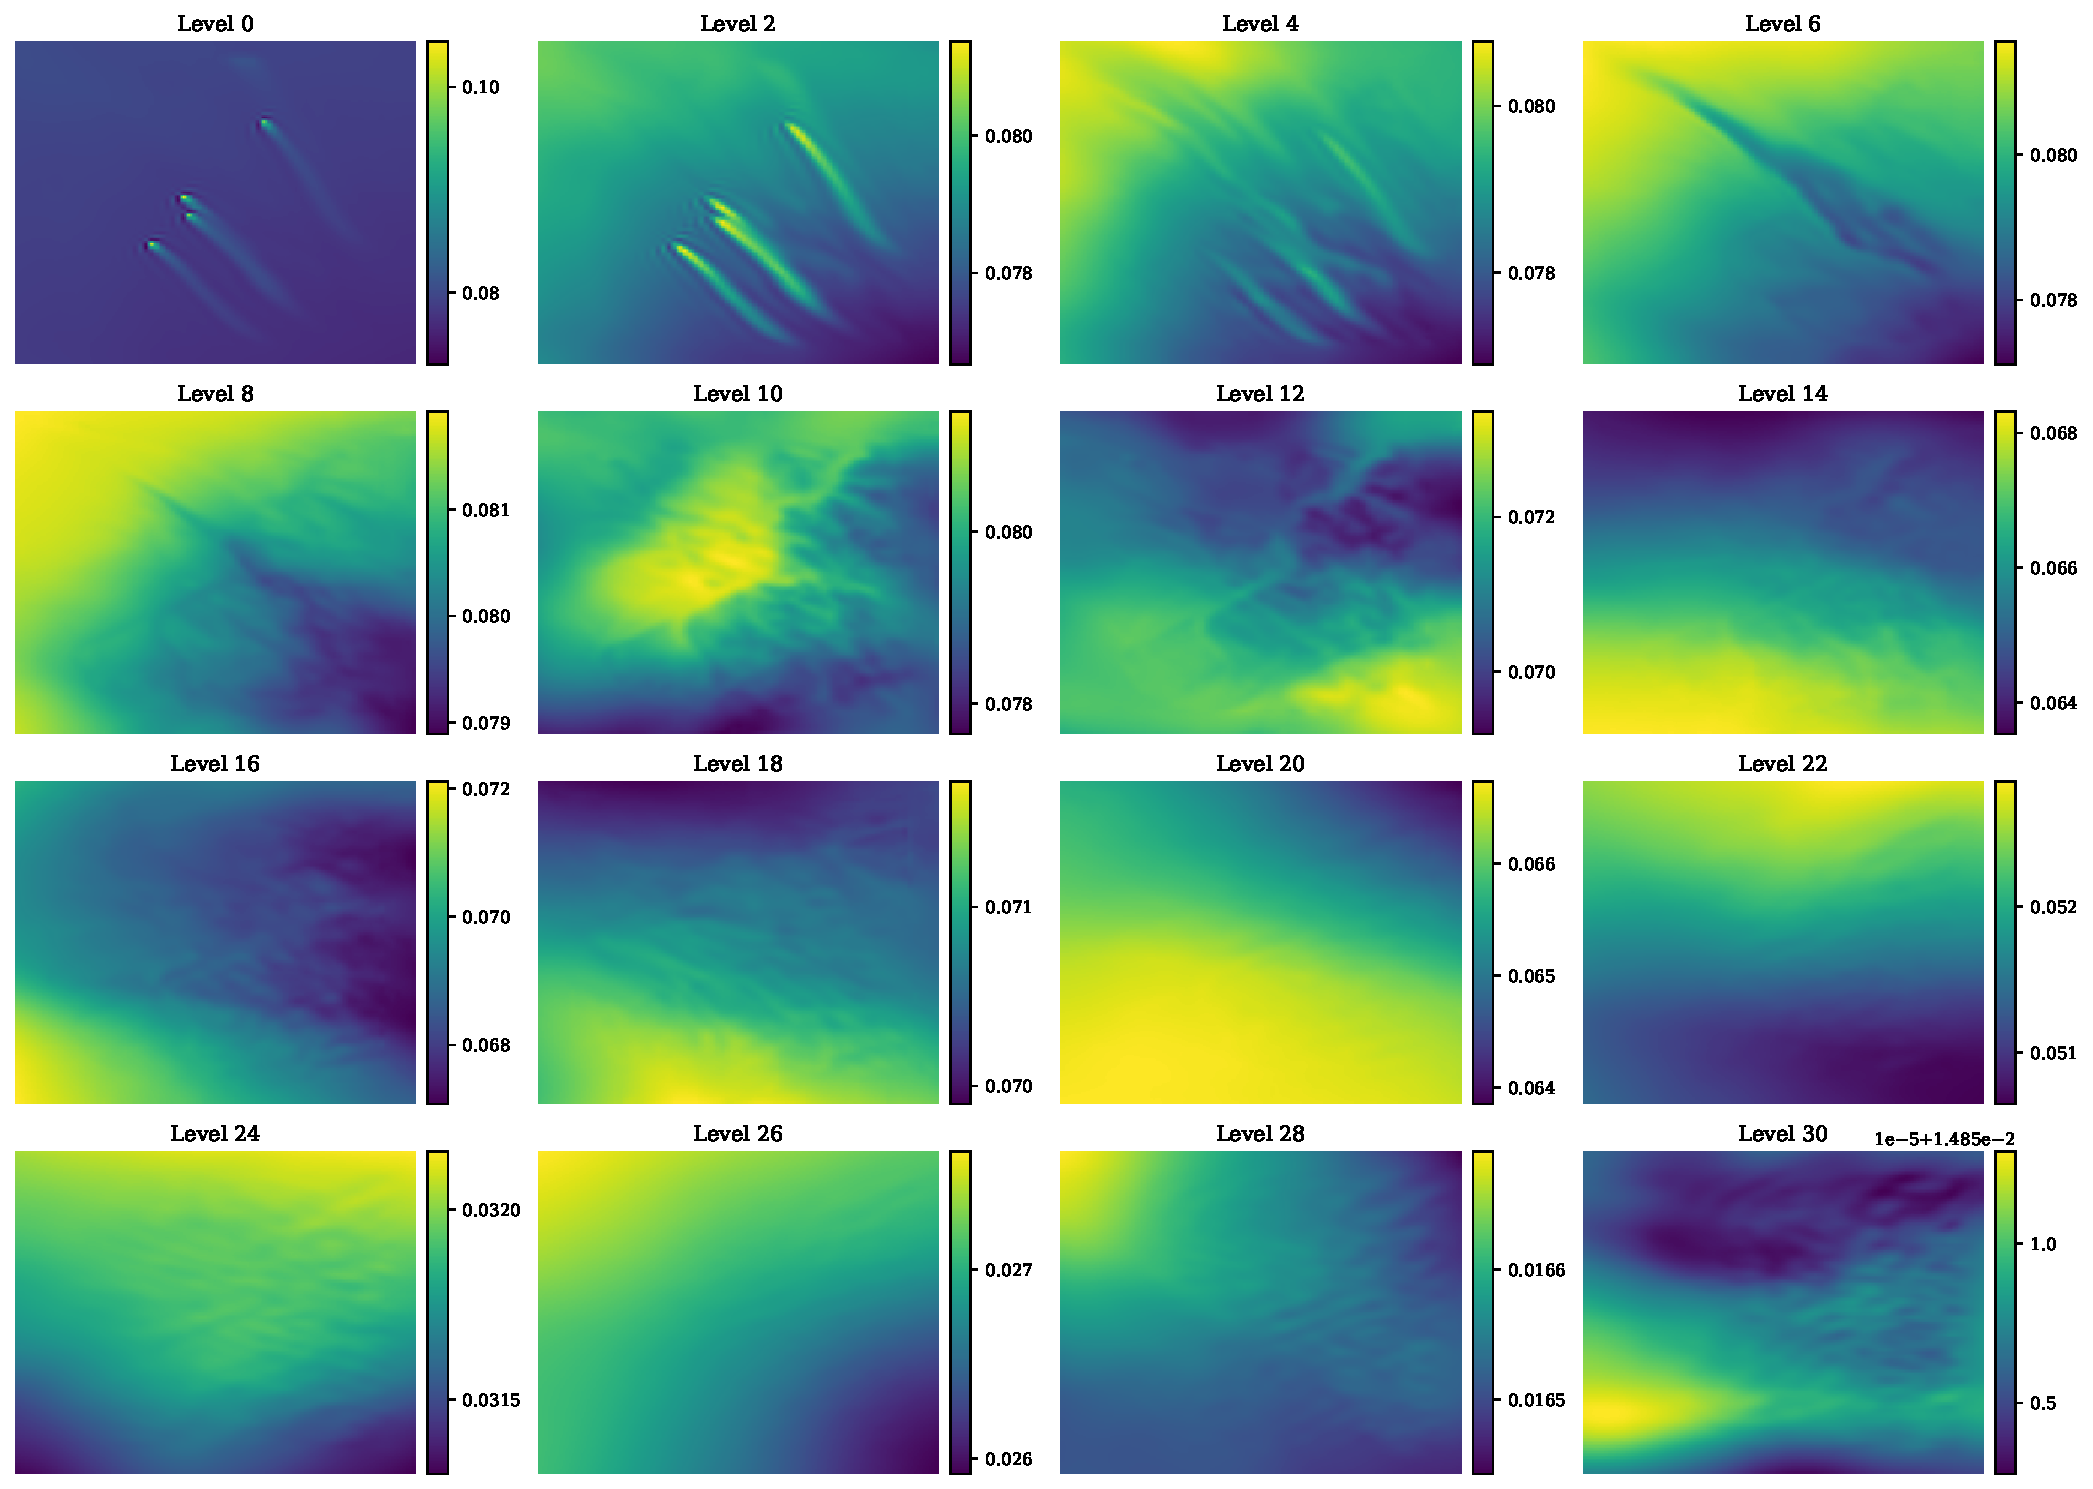
\includegraphics[width=.80\textwidth]{figure_co_levels_32_2.pdf}
  \caption{Spatial distribution of CO concentration at 32 vertical levels (every second level is visualized). Each subfigure represents a horizontal slice of the concentration field. To better visualize spatial features at high altitudes, an independent color scale (local normalization) is used for each level.}
  \label{fig:co_levels}
\end{figure}

\begin{figure}[htbp]
  \centering
  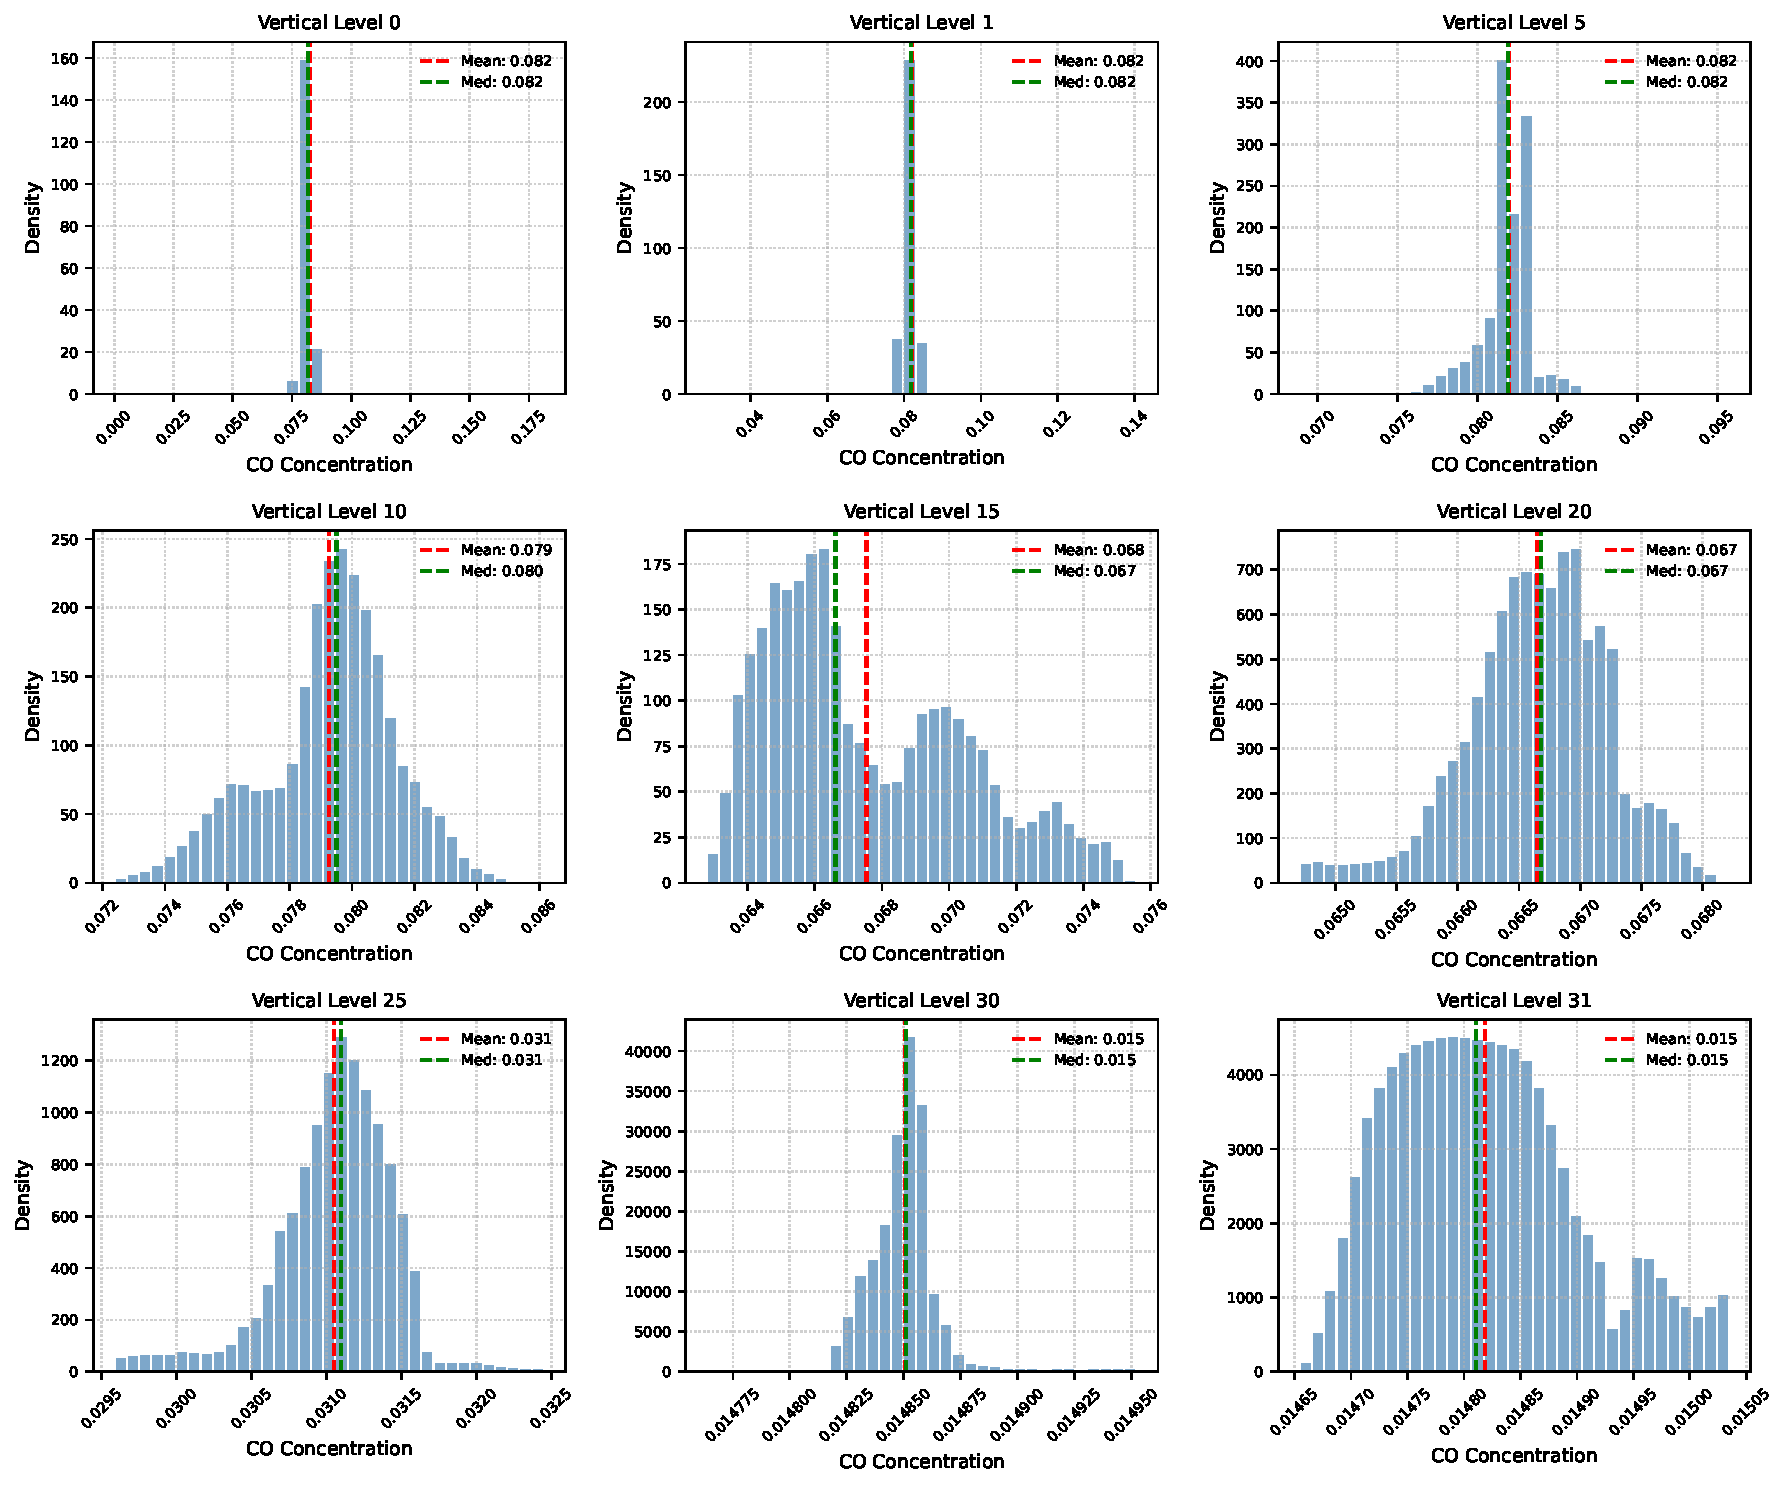
\includegraphics[width=.84\textwidth]{co_concentration_histograms.pdf}
  \caption{Distribution of CO concentrations at selected vertical levels after removing outliers using a $|z|<3$ threshold. The strong level-to-level variability motivates height-wise normalization.}
  \label{fig:co_histograms}
\end{figure}


\section{Methods}

\subsection{Baseline dimensionality-reduction methods}

As baseline comparisons, several classes of dimensionality reduction algorithms were selected. Principal Component Analysis (PCA) and truncated Singular Value Decomposition (truncated SVD) were included as adaptive linear subspace methods. Fixed-basis transform methods were represented by the Discrete Cosine Transform (DCT) and wavelet compression. To assess the effect of spatial approximation, interpolation-based compression was employed. Among tensor formats that preserve multidimensional data structure, the Tensor Train (TT) decomposition was considered. As a representative of nonlinear dimensionality reduction, UMAP was adopted; however, it should be noted that its inverse transform is approximate, which limits its applicability in tasks requiring differentiable inverse modelling. Finally, a plain three-dimensional convolutional autoencoder without attention mechanisms was chosen as the neural-network baseline, allowing the contribution of architectural refinements to be evaluated.

\subsection{3D convolutional autoencoder}

The neural compressor is a symmetric encoder-decoder network based on three-dimensional convolutions. The encoder maps an input field to a latent vector of dimension $d$, while the decoder reconstructs the full field from this latent representation. Each encoder block contains a 3D convolution, a ReLU activation, an optional spatial attention module, and Dropout3D regularization. Decoder blocks use transposed 3D convolutions with the same general pattern.

During deployment in an inverse modelling workflow, the encoder $\mathcal{E}$ provides the compact representation. The decoder $\mathcal{D}$ is required during training and validation because it defines the reconstruction loss and allows the quality of the latent representation to be measured.


\begin{figure}[htbp]
  \centering
  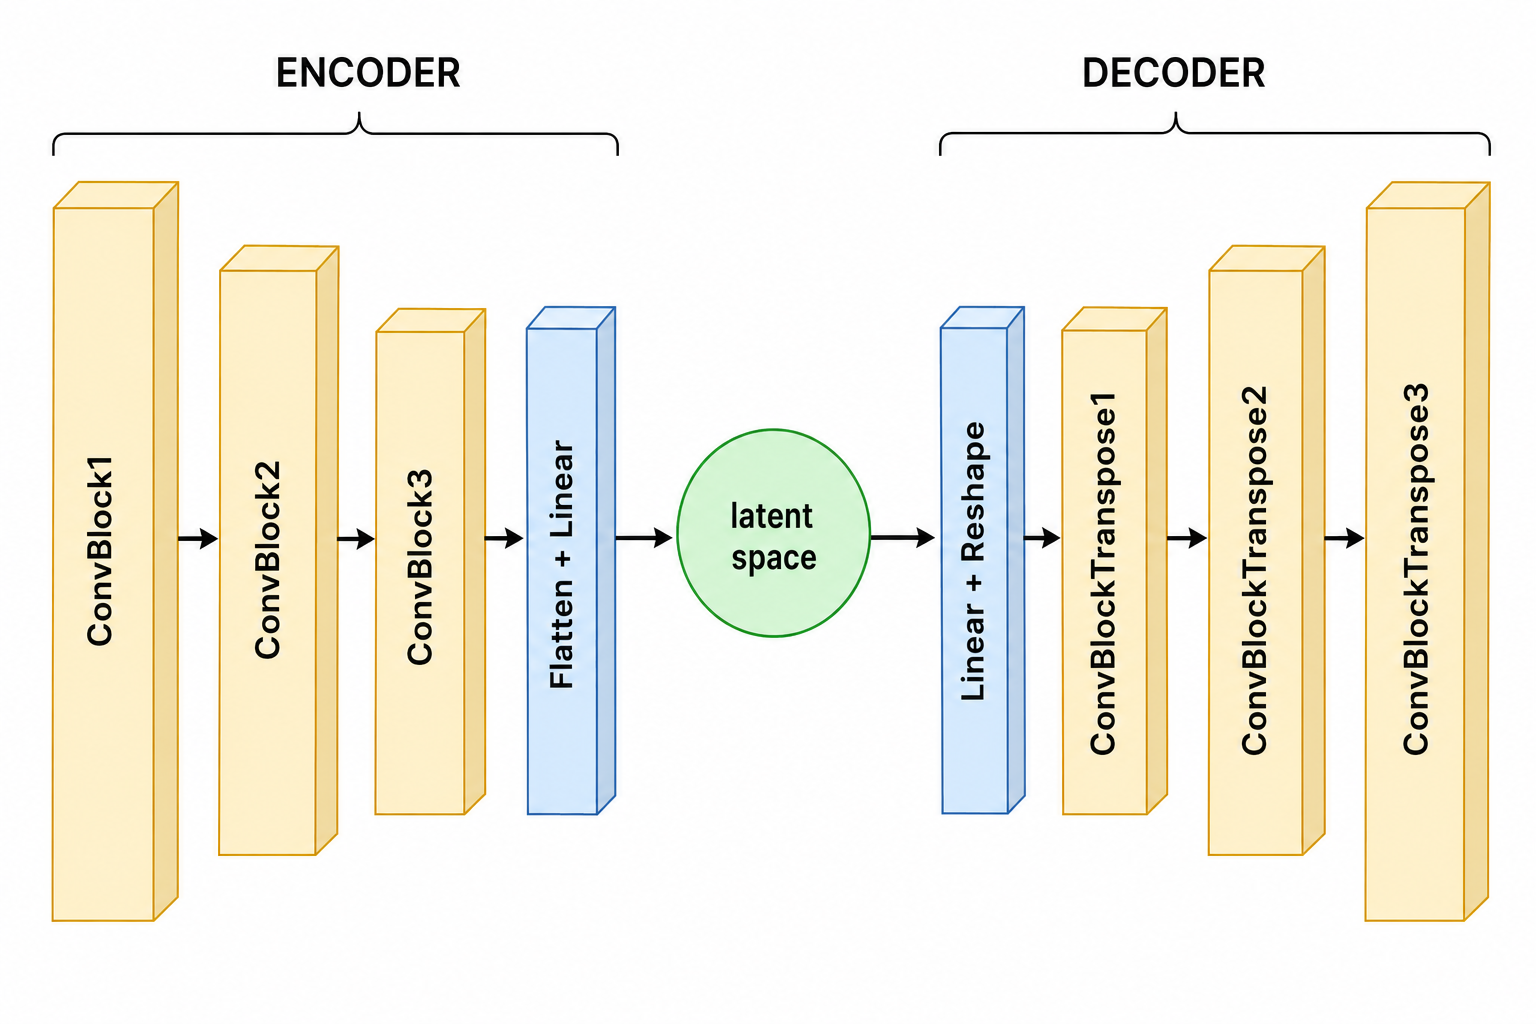
\includegraphics[width=.8\textwidth]{aeshema.png}
  \caption{Architecture of the 3D convolutional autoencoder used for dimensionality reduction of concentration fields.}
  \label{fig:ae_scheme}
\end{figure}

\subsection{SAM3D spatial attention module}

The proposed SAM3D module computes a spatial attention map for a volumetric feature tensor
\begin{equation}
F \in \mathbb{R}^{B \times C \times H_z \times H_y \times H_x},
\end{equation}
where $B$ is the batch size and $C$ is the number of feature channels. Three channel-wise descriptors are calculated at each spatial position of:
\begin{equation}
F_c \in \mathbb{R}^ {H_z \times H_y \times H_x}, \\
\end{equation}


\begin{align}
F_{\mathrm{avg}} &= \frac{1}{C}\sum_{c=1}^{C}F_c, \\
F_{\mathrm{max}} &= \max_{c}F_c, \\
F_{\mathrm{std}} &= \sqrt{\frac{1}{C}\sum_{c=1}^{C}(F_c-F_{\mathrm{avg}})^2}.
\end{align}
These descriptors are concatenated and passed through a 3D convolution followed by a sigmoid activation:
\begin{equation}
A = \sigma\left(\mathrm{Conv3D}\left([F_{\mathrm{avg}},F_{\mathrm{max}},F_{\mathrm{std}}]\right)\right).
\end{equation}
The refined feature tensor is then
\begin{equation}
F_{\mathrm{out}} = F \odot A,
\end{equation}
where $\odot$ is element-wise product

Unlike full self-attention, SAM3D does not form pairwise interactions between all spatial positions. Its computational complexity is therefore linear in the number of grid cells, making it more suitable for volumetric environmental fields.

\begin{figure}[htbp]
  \centering
  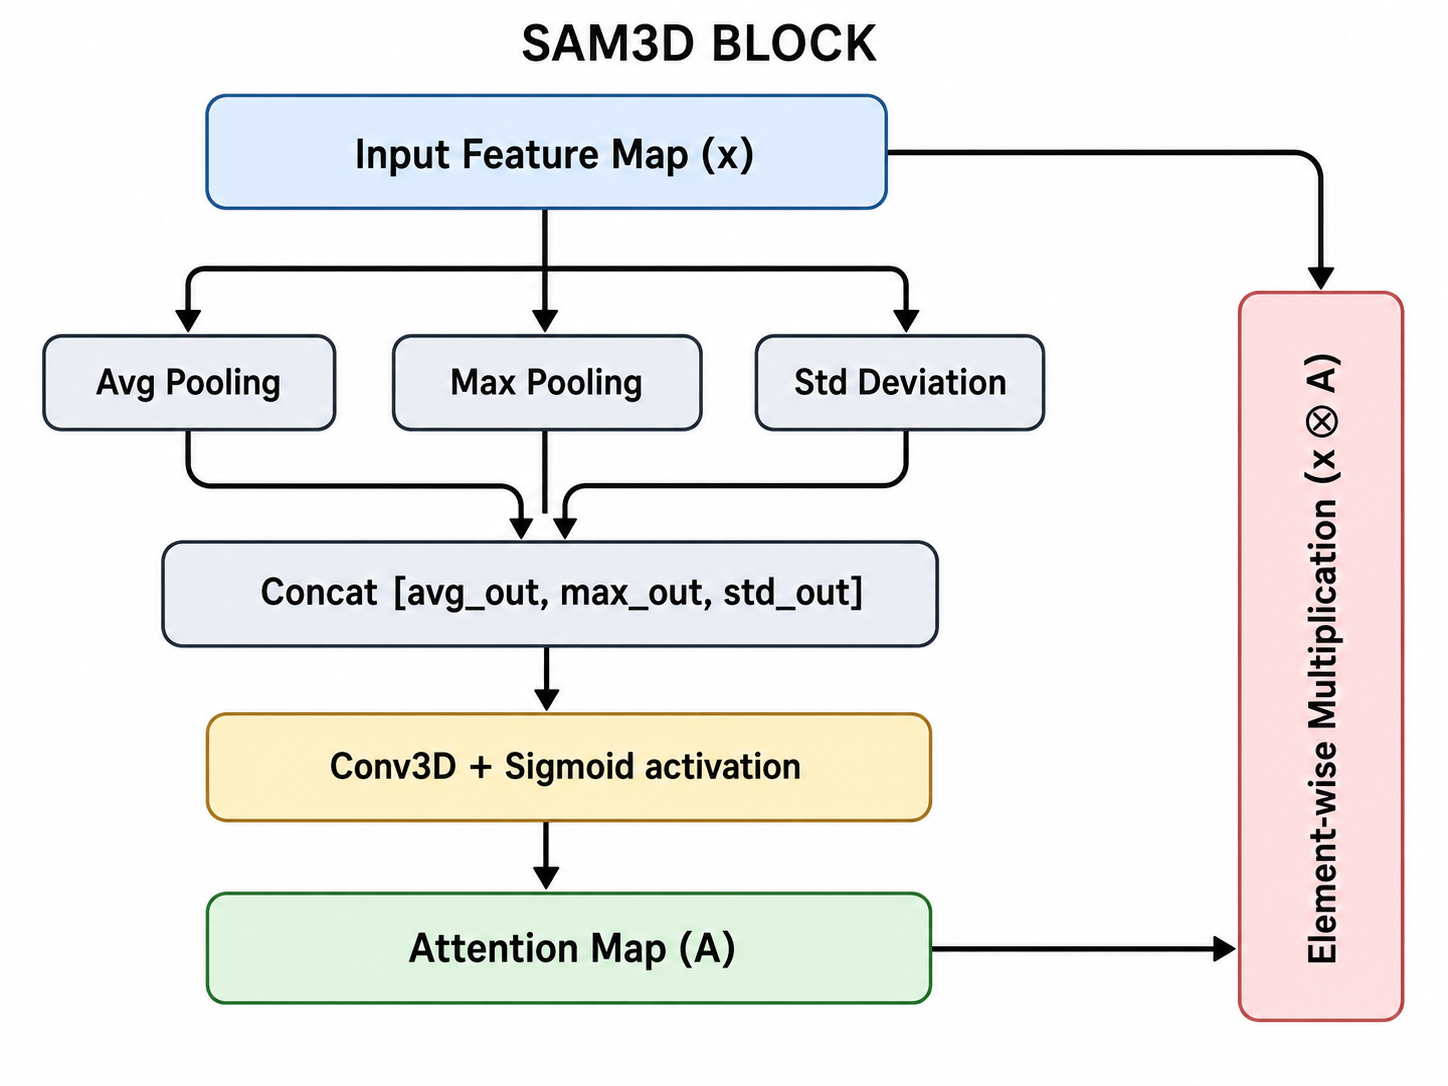
\includegraphics[width=.7\textwidth]{sam.png}
  \caption{SAM3D spatial attention module. Channel-wise mean, maximum, and standard deviation descriptors are combined to generate a volumetric attention map.}
  \label{fig:sam3d_scheme}
\end{figure}


\subsection{Model architecture}

The autoencoder receives a single-channel three-dimensional concentration field of size $32 \times 96 \times 84$, corresponding to the vertical, latitudinal, and longitudinal dimensions, respectively. Separate models were trained using latent dimensions $d \in \{8,16,32,64\}$. Dropout3D with a dropout probability of 0.1 was applied in the encoder and decoder blocks. The proposed model includes the SAM3D spatial-attention module, whereas the plain 3D-CAE baseline uses the same encoder-decoder architecture without attention. This design ensures that the comparison isolates the contribution of the attention mechanism.

\subsection{Training setup}

The neural-network models were trained for a maximum of 100 epochs using a batch size of 32 and an initial learning rate of $10^{-3}$. A weight-decay coefficient of $10^{-6}$ was used for regularization. Early stopping was applied by monitoring the validation loss with a patience of 20 epochs and a minimum improvement threshold of $10^{-4}$. Training was terminated when the validation loss did not improve by at least this threshold during 20 consecutive epochs. The model parameters corresponding to the lowest validation loss were retained for subsequent evaluation. Adam was used as the optimizer. All neural-network experiments were performed on a Linux workstation equipped with an NVIDIA RTX A6000 GPU with 48 GB of memory. The models were implemented in Python 3.12.6 using PyTorch 2.12.1 and CUDA 13.0.

\subsection{Training objective}

The autoencoder was trained using a combined reconstruction loss:
\begin{equation}
\mathcal{L}_{\mathrm{total}} =
\mathcal{L}_{\mathrm{MSE}} + \beta \mathcal{L}_{\mathrm{MAE}},
\end{equation}
where
\begin{equation}
\mathcal{L}_{\mathrm{MSE}} = \frac{1}{n}\sum_{i=1}^{n}(y_i-\hat{y}_i)^2,
\qquad
\mathcal{L}_{\mathrm{MAE}} = \frac{1}{n}\sum_{i=1}^{n}|y_i-\hat{y}_i|.
\end{equation}

MSE penalizes large deviations and supports global field reconstruction, while MAE is less sensitive to outliers and helps reduce excessive smoothing. The coefficient $\beta$ was selected with Optuna \citep{Akiba2019}; the best value in the experiments was $\beta=0.2$. The corresponding total-loss, MAE, and MSE training curves are shown in Figure~\ref{fig:loss_curves}, as we can see, the loss function decreases on both the training set and the validation set, which indicates the absence of overfitting.
\begin{figure}[htbp]
  \centering
  \begin{subfigure}[b]{0.6\textwidth}
    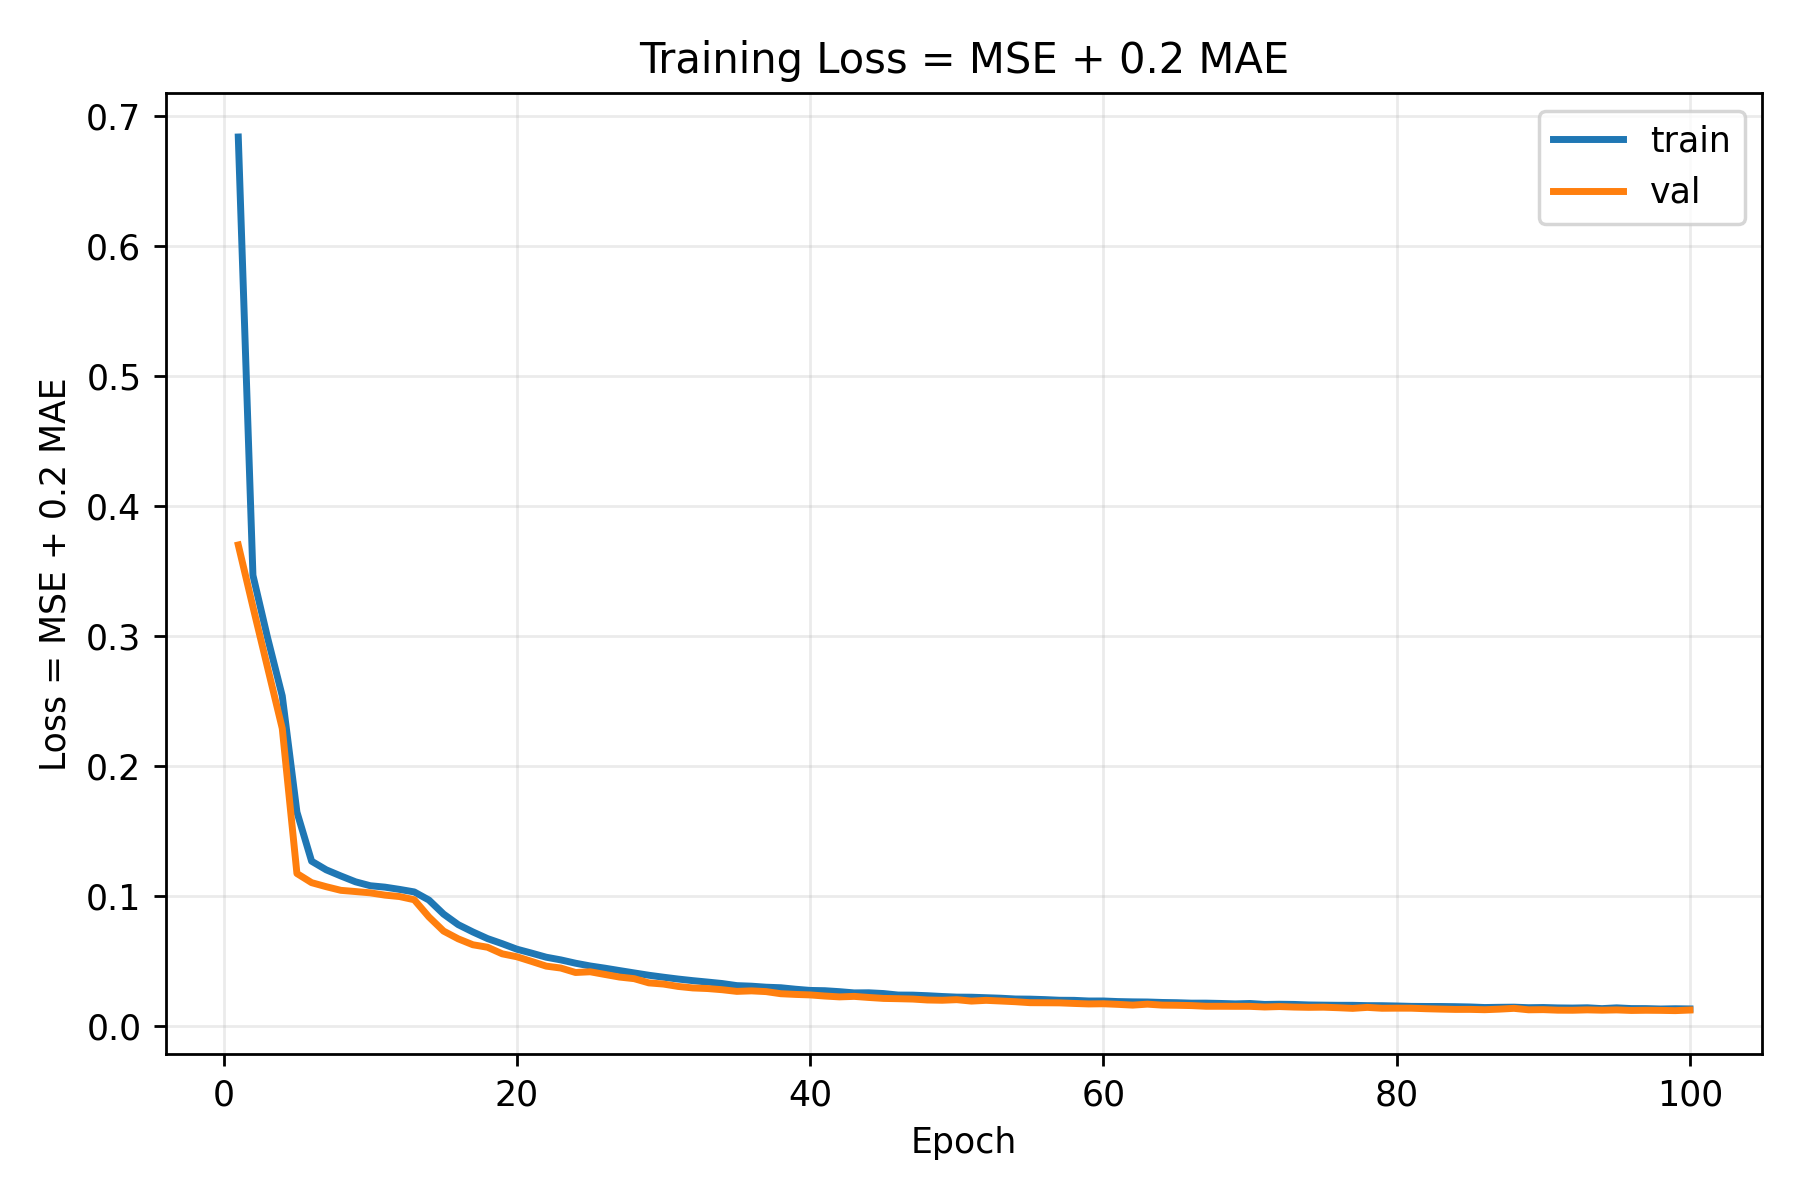
\includegraphics[width=\textwidth]{loss_new.png}
    \caption{Total loss}
  \end{subfigure}
  \hfill
  \begin{subfigure}[b]{0.6\textwidth}
    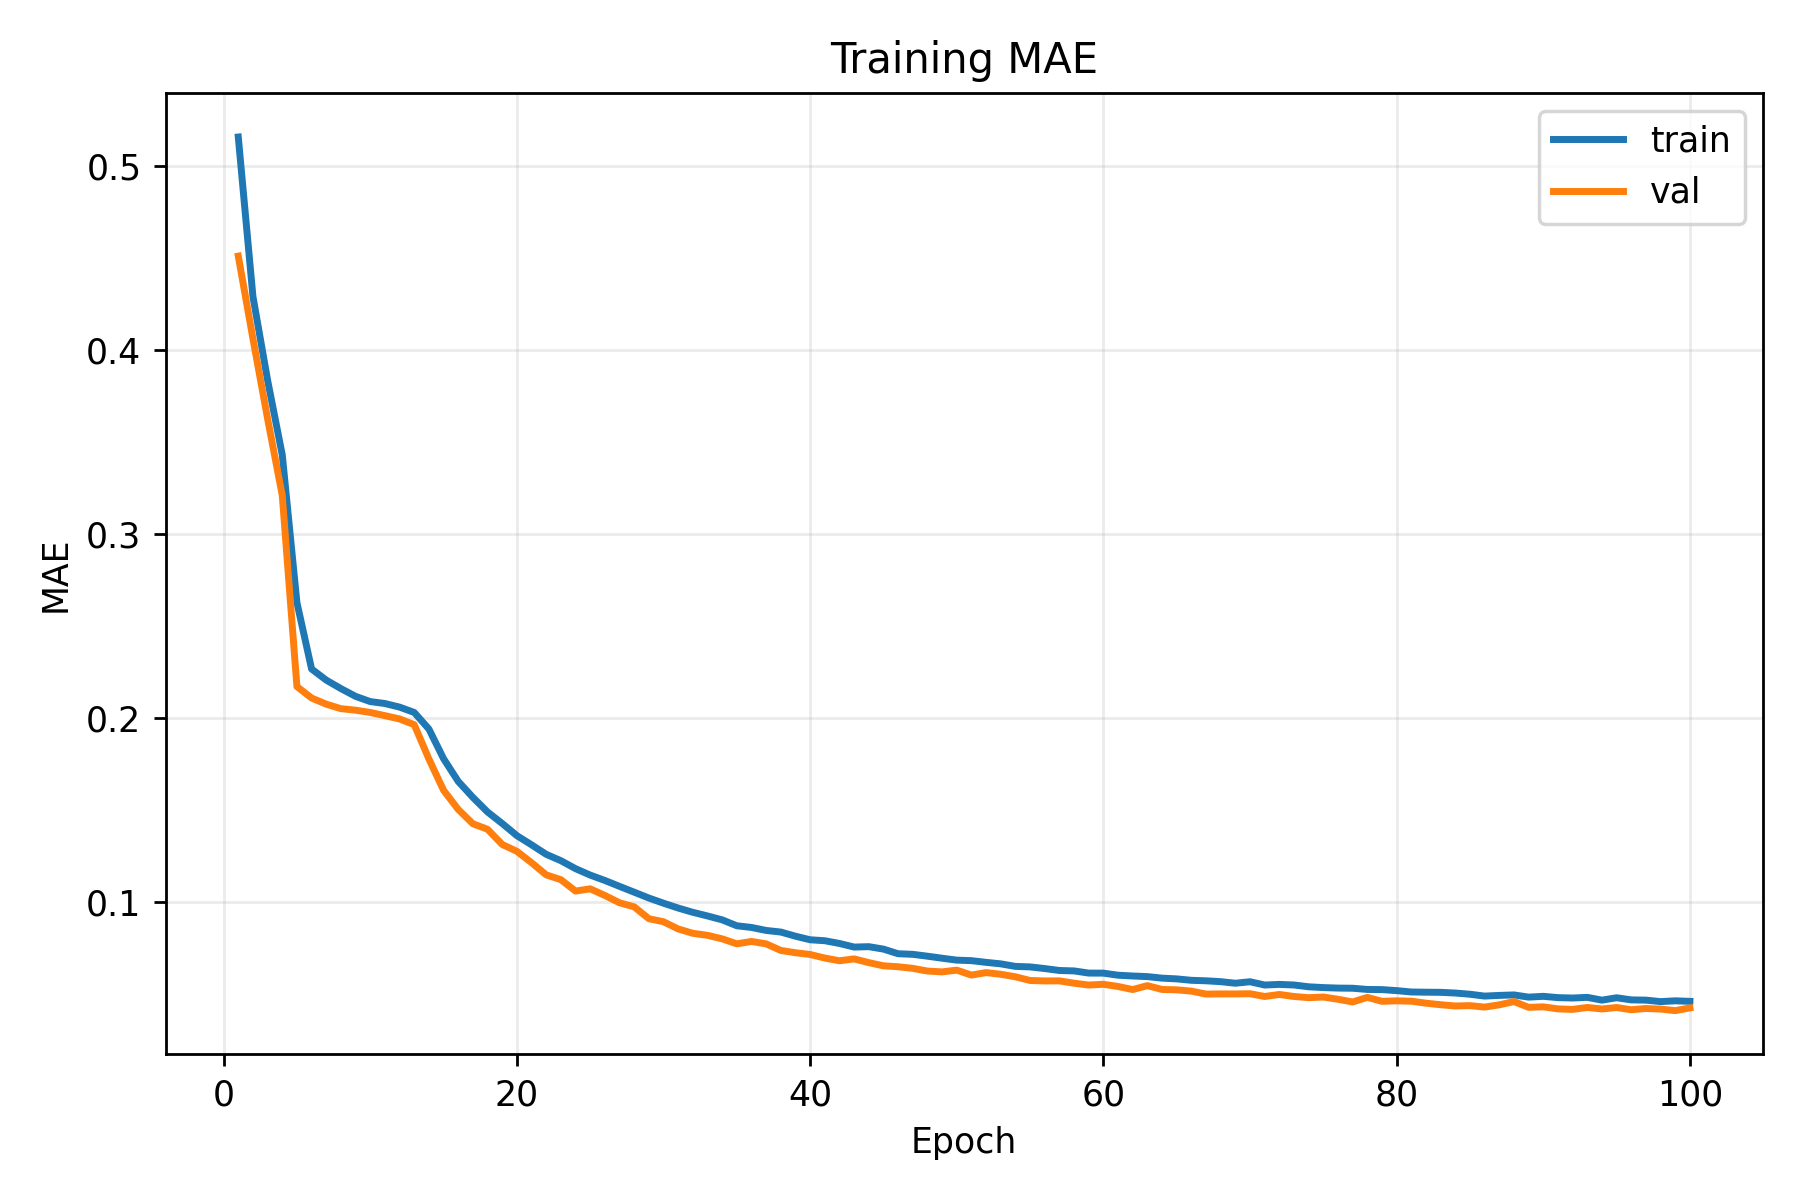
\includegraphics[width=\textwidth]{mae_new.png}
    \caption{MAE}
  \end{subfigure}
  \hfill
  \begin{subfigure}[b]{0.6\textwidth}
    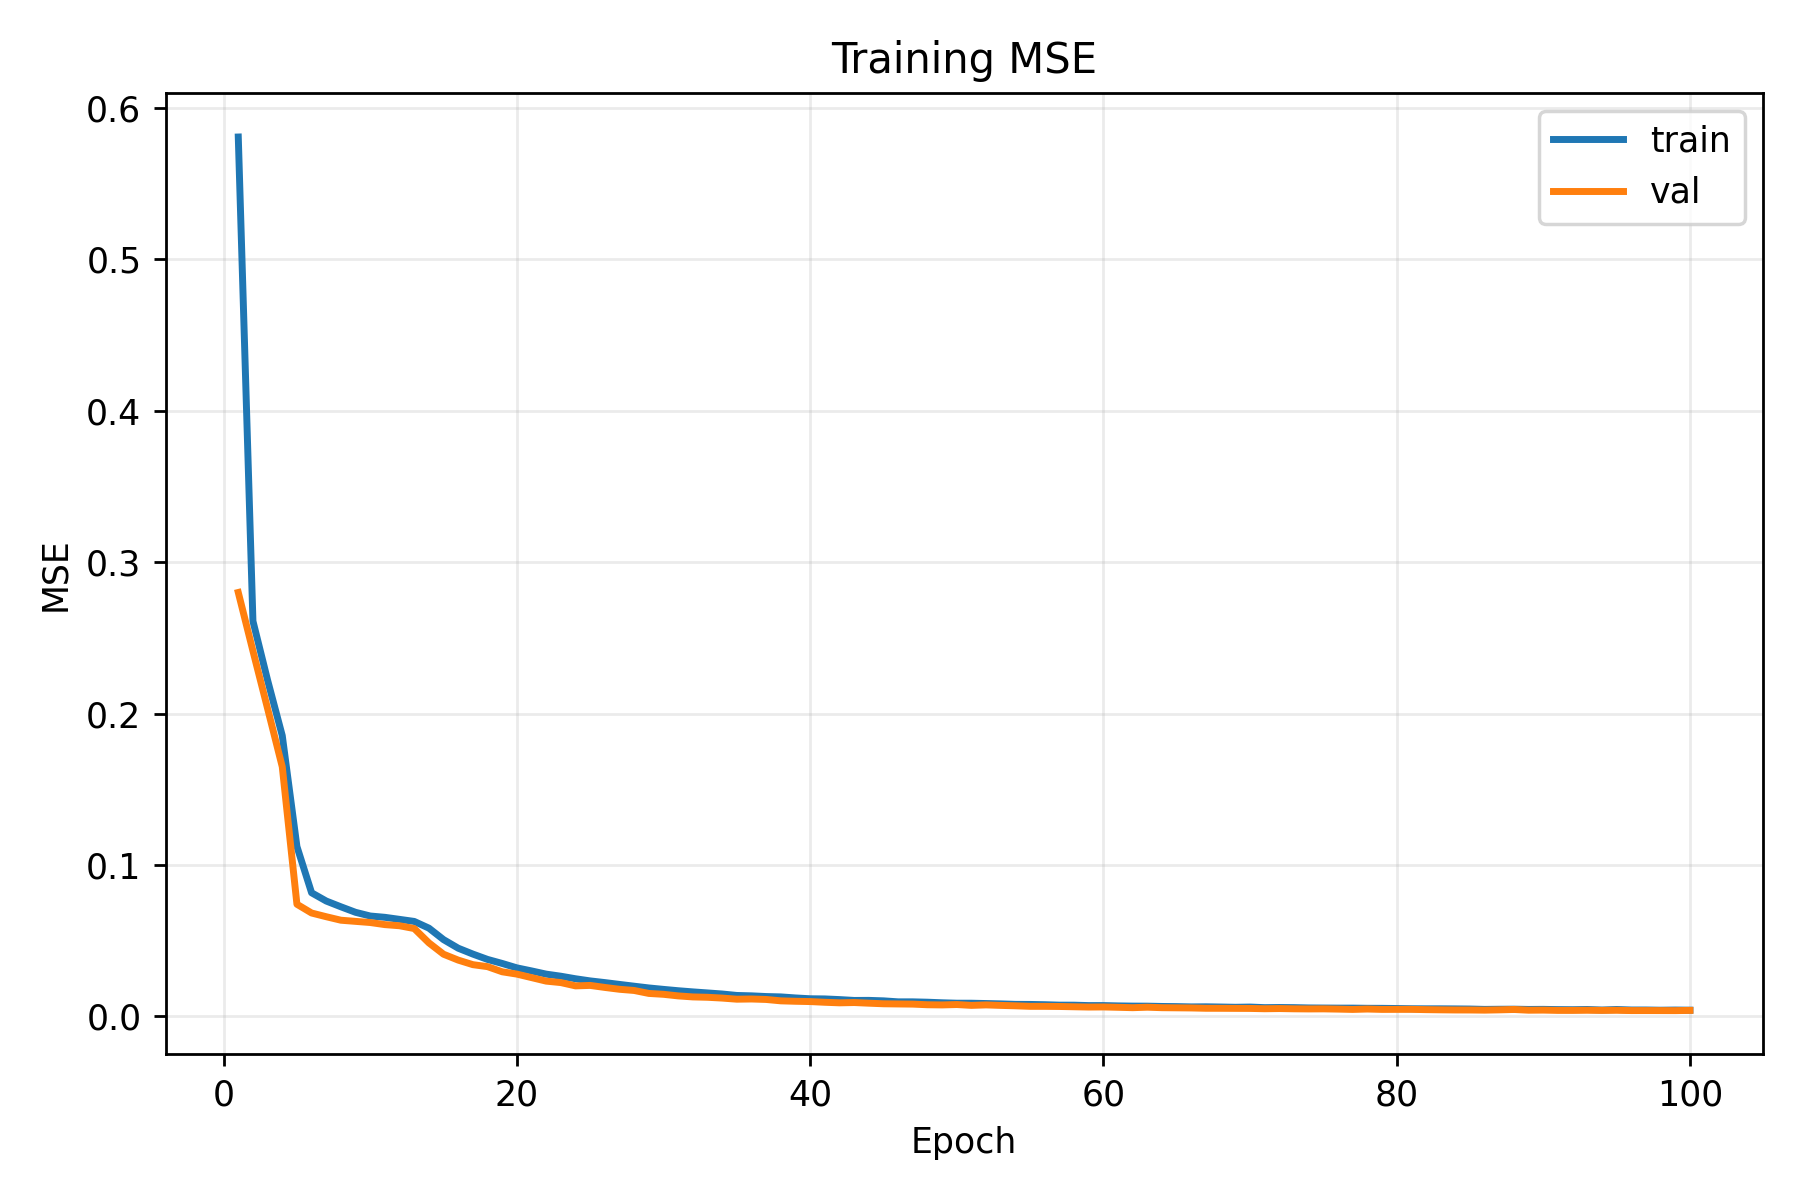
\includegraphics[width=\textwidth]{mse_new.png}
    \caption{MSE}
  \end{subfigure}
  \caption{Training curves for the 3D convolutional autoencoder (for a latent dimension of 32).}
  \label{fig:loss_curves}
\end{figure}


In order to verify the stability of the proposed model, we additionally performed 5-fold cross-validation, which confirmed that the training procedure yields consistent results across different data splits. The resulting distribution of the validation MSE is shown in Figure~\ref{fig:cv_mse}.

\begin{figure}[htbp]
  \centering
  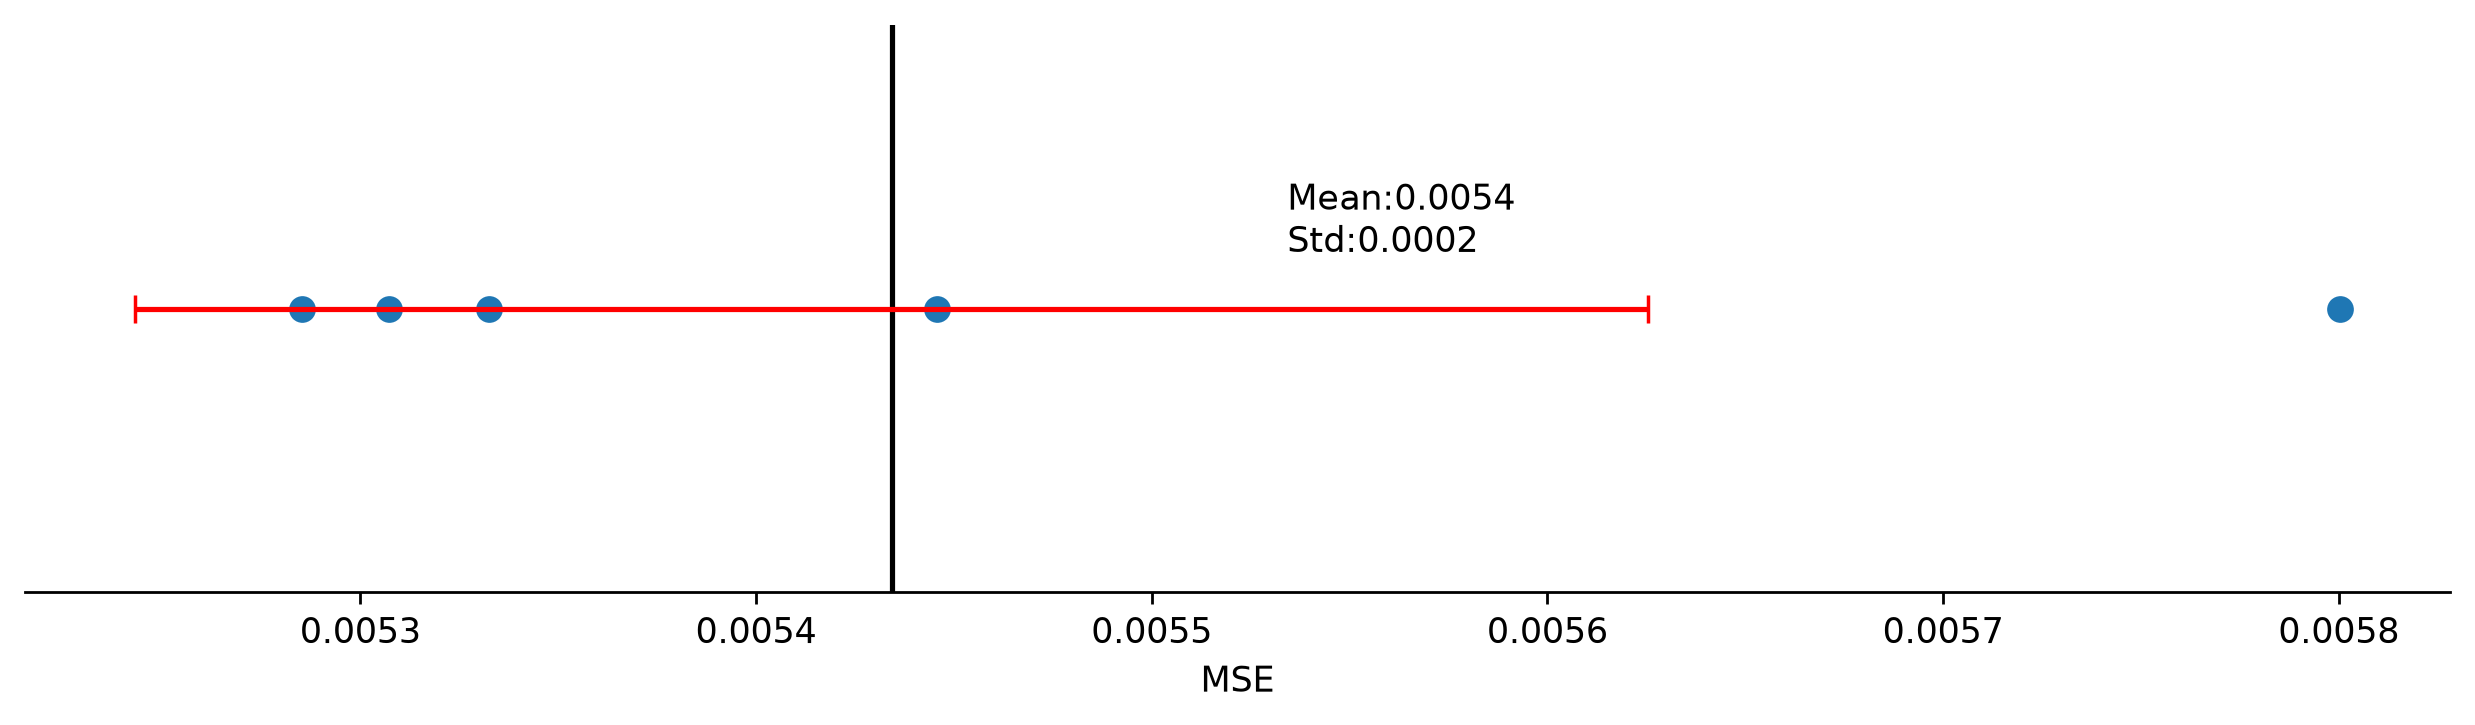
\includegraphics[width=.9\textwidth]{cv_mse_distribution.png}
  \caption{Distribution of cross-validation MSE for a latent dimension of 32, where the red line represents the standard deviation and the dots represent error values across folds.}
  \label{fig:cv_mse}
\end{figure}

\subsection{Differentiability and Jacobian analysis}

The proposed encoder--decoder mapping is a composition of operations supported by automatic differentiation frameworks such as PyTorch \citep{Paszke2019}. Convolutions and transposed convolutions are linear with respect to the input for fixed network parameters. Sigmoid activations are differentiable, whereas ReLU activations, maximum operations, and related pooling operations are differentiable almost everywhere and admit subgradients at their non-smooth points \citep{Rumelhart1986,LeCun2015,Bottou2016}. Consequently, the trained network can be incorporated into a differentiable inverse-modelling workflow, with the practical caveat that the sensitivity and conditioning of the corresponding Jacobian should be monitored.

To quantify the local sensitivity of the latent representation to perturbations in the input concentration field, the Jacobian of the trained encoder was analysed. Let
\begin{equation}
\mathcal{E}_{\theta}\colon \mathbb{R}^{D} \rightarrow \mathbb{R}^{d}
\end{equation}
denote the encoder with fixed trained parameters $\theta$, where $D$ is the dimensionality of the input concentration field and $d$ is the latent-space dimension. For an input field $\mathbf{x}$, the encoder Jacobian is defined as
\begin{equation}
J_{\mathcal{E}}(\mathbf{x})
=
\frac{\partial \mathcal{E}_{\theta}(\mathbf{x})}
{\partial \mathbf{x}}
\in \mathbb{R}^{d \times D}.
\label{eq:encoder_jacobian}
\end{equation}

The derivatives were calculated for held-out concentration fields using automatic differentiation in PyTorch. Two matrix norms were considered. The spectral norm,
\begin{equation}
\left\lVert J_{\mathcal{E}}(\mathbf{x}) \right\rVert_{2}
=
\sigma_{\max}\!\left(J_{\mathcal{E}}(\mathbf{x})\right),
\label{eq:jacobian_spectral_norm}
\end{equation}
characterizes the maximum local amplification of an input perturbation by the encoder. The Frobenius norm,
\begin{equation}
\left\lVert J_{\mathcal{E}}(\mathbf{x}) \right\rVert_{\mathrm{F}}
=
\left(\sum_{i=1}^{d}
\sum_{j=1}^{D}
\left|
\frac{\partial \mathcal{E}_{\theta,i}(\mathbf{x})}
{\partial x_j}
\right|^{2}
\right)^{1/2},
\label{eq:jacobian_frobenius_norm}
\end{equation}
provides an aggregate measure of sensitivity over all input and latent dimensions.

The resulting distributions of the spectral and Frobenius norms are shown in Figure~\ref{fig:jacobian_norm}. This analysis characterizes the local sensitivity of the encoder with respect to perturbations of the normalized input fields. The reported norms therefore describe the neural encoder itself and do not include the frame-wise min--max normalization or the inverse-scaling procedure. These results should be interpreted as empirical sensitivity diagnostics rather than as a direct proof of the stability of a complete inverse-modelling algorithm.


\begin{figure}[htbp]
  \centering
  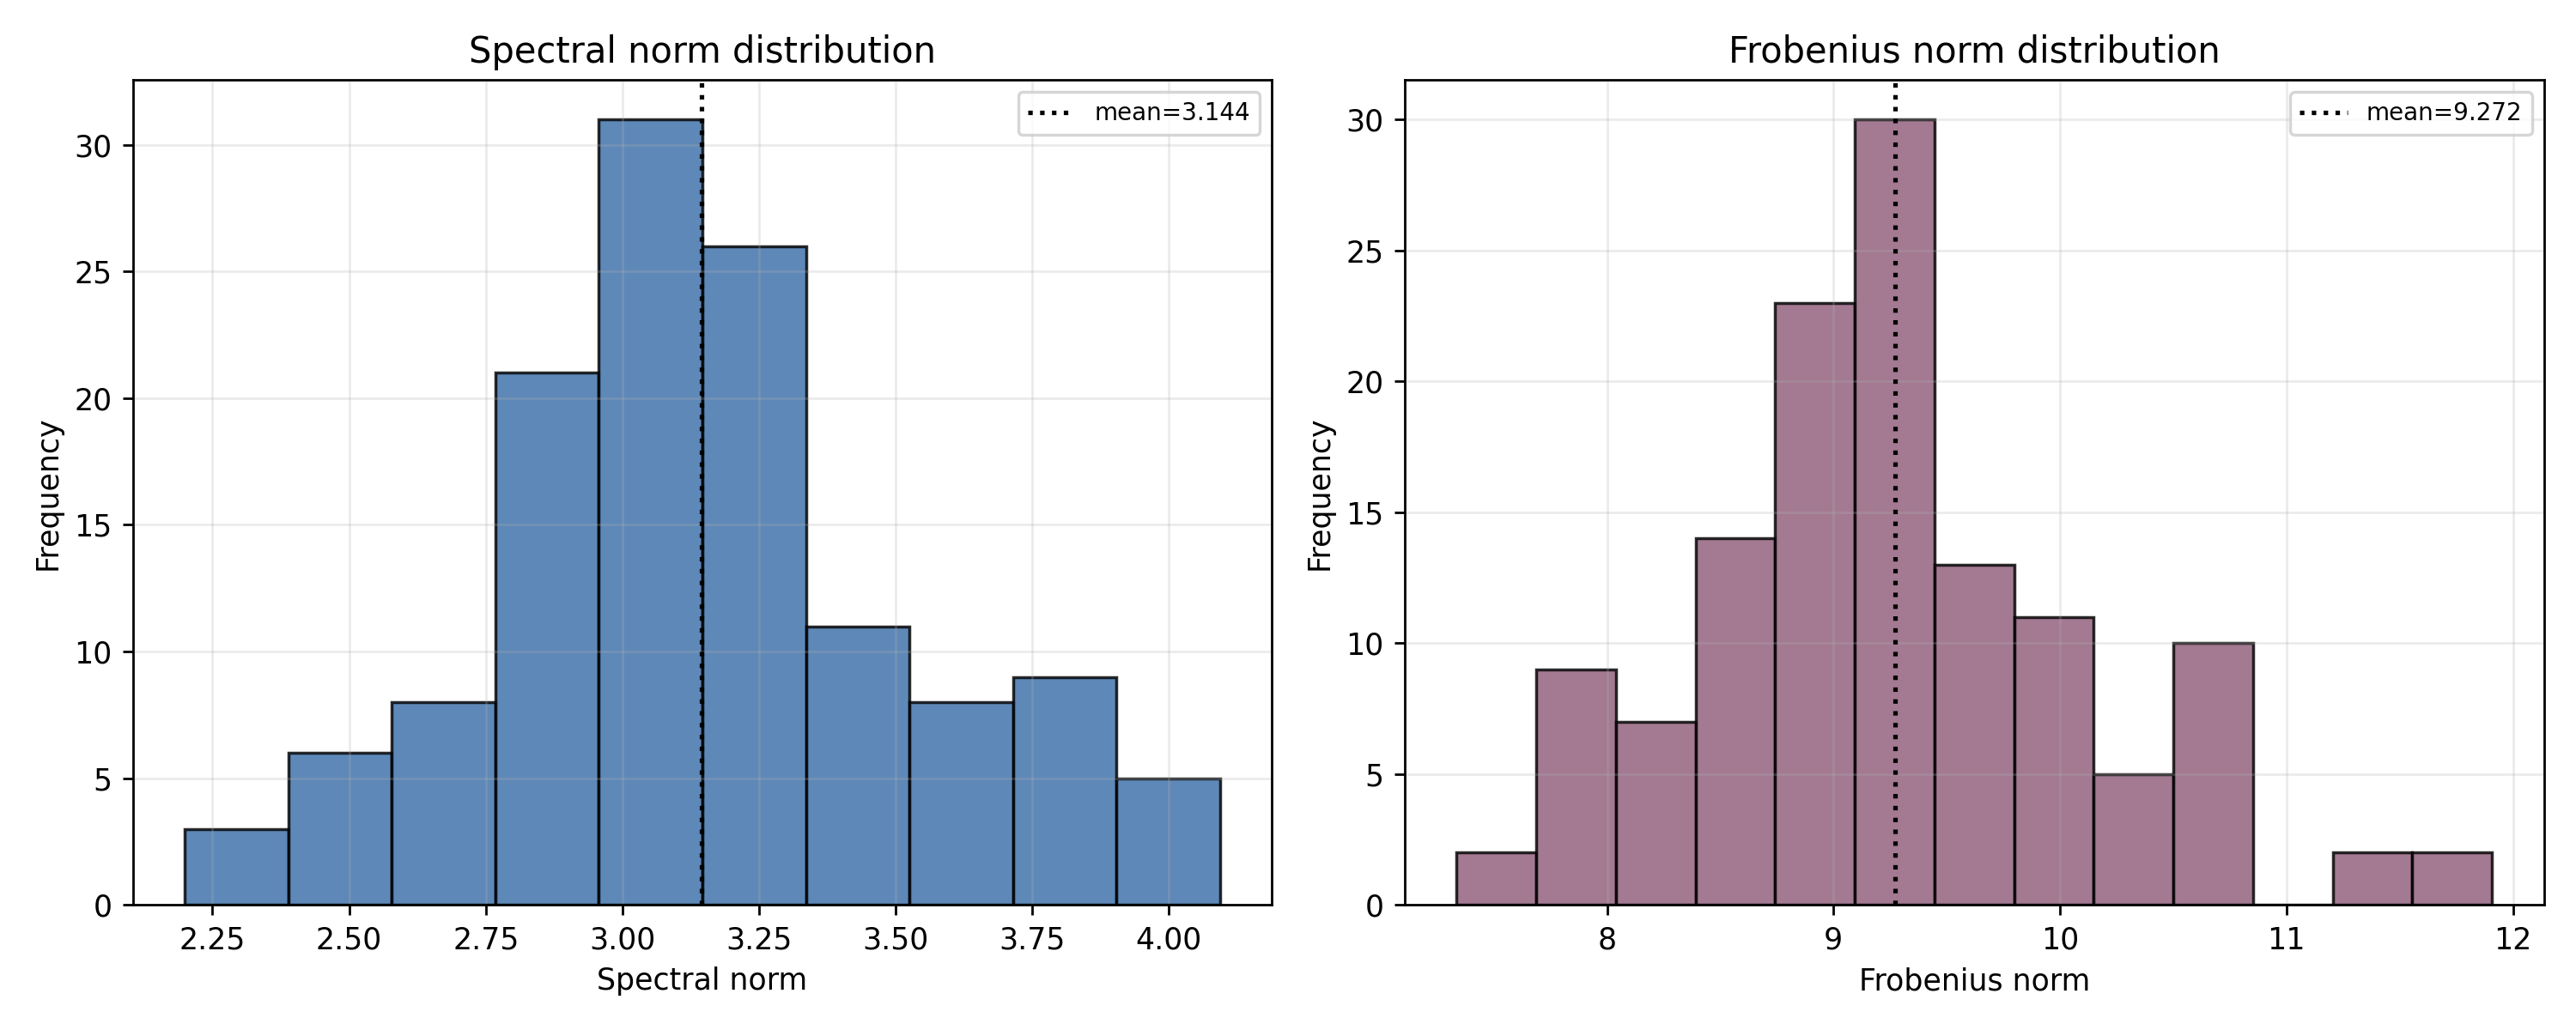
\includegraphics[width=.9\textwidth]{jacobian_norm_distributions.png}
  \caption{Distribution of the spectral and Frobenius norms of the Jacobian matrix for the trained autoencoder.}
  \label{fig:jacobian_norm}
\end{figure}

\section{Results}

\begin{table}[htbp]
\caption{MSE for different latent dimensions. The best value among methods with a fixed number of components is highlighted.}
\label{tab:mse_by_components}
\centering
\begin{tabular}{lrrrr}
\toprule
Method & 8 & 16 & 32 & 64 \\
\midrule
3D-CAE & 0.0123 & 0.0118 & 0.0069 & 0.0065 \\
3D-CAE-SAM3D & 0.0102 & \textbf{0.0074} & \textbf{0.0053} & \textbf{0.0045} \\
PCA & 0.0328 & 0.0236 & 0.0145 & 0.0079 \\
DCT & 0.0355 & 0.0250 & 0.0163 & 0.0100 \\
Wavelet & 0.0820 & 0.0588 & 0.0509 & 0.0441 \\
Interpolation & 0.2136 & 0.2114 & 0.1057 & 0.1058 \\
Truncated SVD & 0.0341 & 0.0242 & 0.0147 & 0.0079 \\
Random projection & 0.2520 & 0.2520 & 0.2520 & 0.2520 \\
UMAP & \textbf{0.0082} & 0.0087 & 0.0083 & 0.0085 \\
\bottomrule
\end{tabular}
\end{table}

\begin{table}[htbp]
\caption{Relative $L_2$ error for different latent dimensions.}
\label{tab:l2_by_components}
\centering
\begin{tabular}{lrrrr}
\toprule
Method & 8 & 16 & 32 & 64 \\
\midrule
3D-CAE & 0.2208 & 0.2166 & 0.1660 & 0.1610 \\
3D-CAE-SAM3D & 0.2009 & \textbf{0.1710} & \textbf{0.1453} & \textbf{0.1337} \\
PCA & 0.3607 & 0.3062 & 0.2397 & 0.1771 \\
DCT & 0.3752 & 0.3148 & 0.2545 & 0.1992 \\
Wavelet & 0.5703 & 0.4828 & 0.4492 & 0.4182 \\
Interpolation & 0.9206 & 0.9158 & 0.6476 & 0.6479 \\
Truncated SVD & 0.3676 & 0.3101 & 0.2416 & 0.1774 \\
Random projection & 1.0000 & 1.0000 & 0.9999 & 0.9999 \\
UMAP & \textbf{0.1799} & 0.1857 & 0.1809 & 0.1835 \\
\bottomrule
\end{tabular}
\end{table}

\begin{table}[htbp]
\caption{SSIM for different latent dimensions.}
\label{tab:ssim_by_components}
\centering
\begin{tabular}{lrrrr}
\toprule
Method & 8 & 16 & 32 & 64 \\
\midrule
3D-CAE & 0.6030 & 0.6423 & 0.7351 & 0.7384 \\
3D-CAE-SAM3D & 0.6213 & 0.6719 & 0.7469 & 0.7715 \\
PCA & 0.5921 & 0.6261 & 0.6654 & 0.7142 \\
DCT & 0.5471 & 0.5773 & 0.6119 & 0.6522 \\
Wavelet & 0.4018 & 0.4491 & 0.4542 & 0.4636 \\
Interpolation & 0.2136 & 0.2230 & 0.4353 & 0.4312 \\
Truncated SVD & 0.5871 & 0.6237 & 0.6641 & 0.7136 \\
Random projection & 0.0194 & 0.0193 & 0.0190 & 0.0184 \\
UMAP & \textbf{0.8361} & \textbf{0.8294} & \textbf{0.8332} & \textbf{0.8311} \\
\bottomrule
\end{tabular}
\end{table}

\begin{table}[htbp]
\caption{Tensor-train SVD results for different tensor ranks.}
\label{tab:tt_svd}
\centering
\begin{tabular}{lrrrrr}
\toprule
Ranks & Compressed size & Compression ratio & MSE & Relative $L_2$ & SSIM \\
\midrule
$(2,4)$ & 1168 & 220.93 & 0.0169 & 0.2589 & 0.6435 \\
$(4,8)$ & 3872 & 66.64 & 0.0069 & 0.1649 & 0.7190 \\
$(8,8)$ & 7072 & 36.49 & 0.0026 & 0.1007 & 0.8032 \\
$(8,16)$ & 13888 & 18.58 & 0.0023 & 0.0954 & 0.8273 \\
$(16,16)$ & 26432 & 9.76 & 0.0005 & 0.0449 & 0.9262 \\
\bottomrule
\end{tabular}
\end{table}

The SAM3D autoencoder outperforms the plain 3D-CAE at every tested latent dimension. At 64 components, the SAM3D model achieves an MSE of 0.0045 and a relative $L_2$ error of 0.1337, surpassing PCA, DCT, and truncated SVD\@. UMAP yields high SSIM values but falls behind our architecture at larger dimensions (16, 32, 64). Moreover, the results show that increasing the number of compression components does not guarantee an improvement in reconstruction accuracy, and the inverse mapping raises additional concerns. Tensor-train SVD achieves high accuracy at larger ranks, but it is parameterized by tensor ranks rather than by a direct latent-vector dimension and therefore represents a different compression trade-off. Overall, the lower MSE and relative $L_2$ error obtained by the SAM3D autoencoder indicate improved reconstruction accuracy compared with the plain 3D-CAE and the main linear baselines. The higher SSIM values further indicate a closer structural similarity between the original and reconstructed concentration fields.



\begin{figure}[htbp]
  \centering
  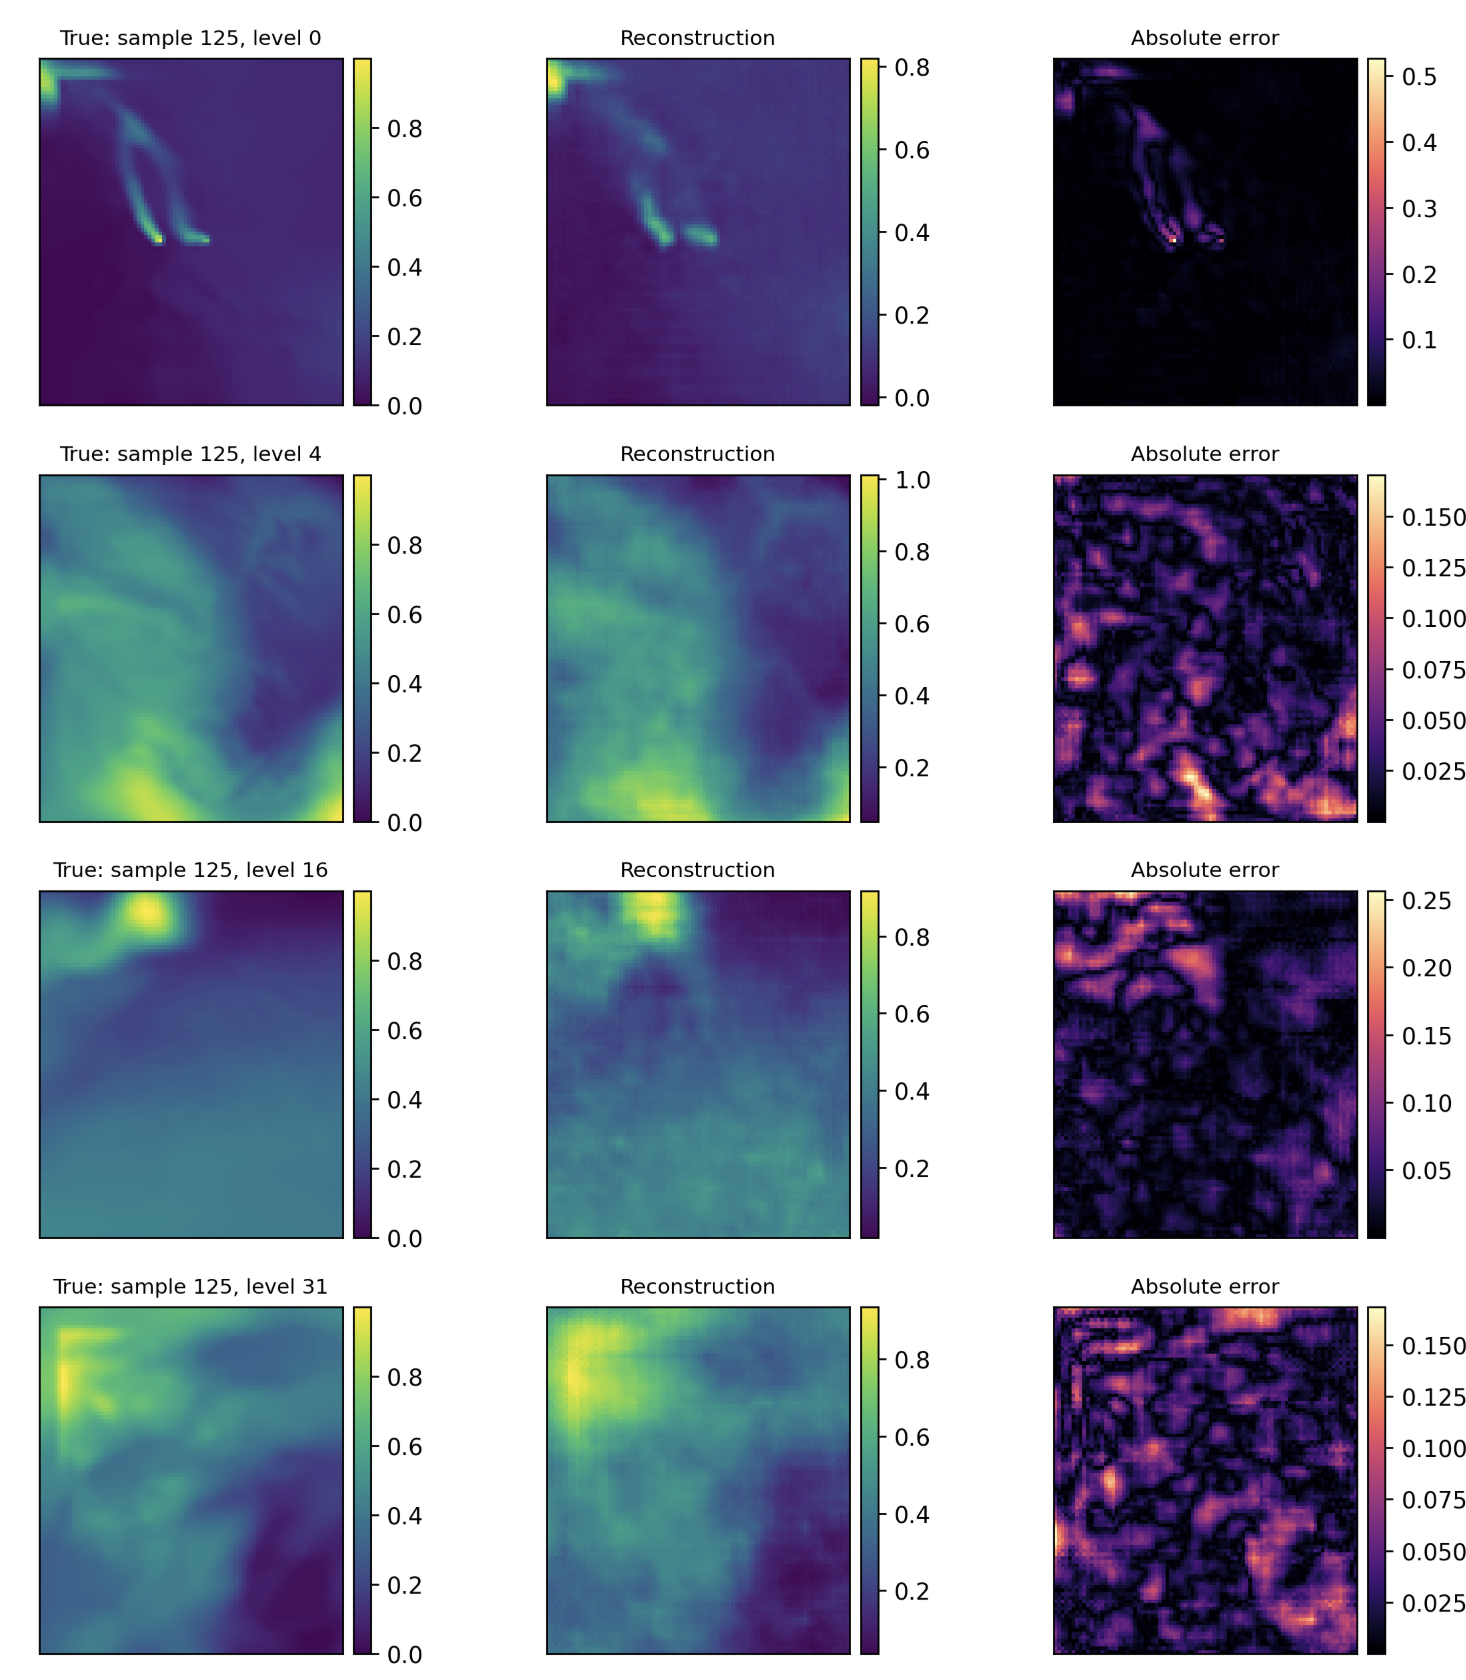
\includegraphics[width=.94\textwidth]{example.png}
  \caption{Example reconstruction using the 3D-CAE-SAM3D model for a validation sample. Lower, middle, and upper vertical levels are shown.}
  \label{fig:height_comparison}
\end{figure}

\section{Discussion}

The results support the usefulness of lightweight spatial attention for environmental model-output compression. Concentration fields generated by urban pollution scenarios are spatially heterogeneous: point sources, transport patterns, and boundary-layer structure lead to localized high-gradient regions. A plain convolutional autoencoder processes these structures through local filters, but it does not explicitly reweight spatial positions according to their reconstruction importance. SAM3D adds this capability with a small computational overhead and without the quadratic memory cost of full self-attention.
The broader significance of this work is that the proposed compressor serves as a software component between detailed environmental simulators and inverse modeling algorithms. It can reduce the dimensionality of model output before sensitivity operator construction, data assimilation, source inversion, or surrogate model fitting. The method is not tied exclusively to CO: the same approach can be applied to other gridded atmospheric tracers, provided that representative simulations are available for training and validation.

The present study focuses specifically on this preliminary dimensionality-reduction stage. Before compressed representations can be incorporated into an inverse-modelling algorithm, it is necessary to determine how strongly atmospheric concentration fields can be compressed, which spatial structures are lost during reconstruction, and which methods provide the most favourable balance between compression and accuracy. The influence of the resulting representations on source inversion and parameter-estimation accuracy is outside the scope of the present paper and will be investigated separately.
Several limitations remain. First, the experiments are based on a regional dataset for Novosibirsk, and transfer to other cities, seasons, meteorological regimes, or pollutants should be tested explicitly. Second, the current evaluation focuses on reconstruction metrics; future work should measure the effect of compression on the final inverse problem, for example source-location accuracy or emission-rate recovery. Third, while differentiability is supported by the computational graph, the conditioning of the encoder and decoder Jacobians should be monitored when the method is coupled to variational methods.

\section{Conclusions}
The development of efficient compression algorithms is essential for inverse modeling applications, where multiple solutions of forward and adjoint problems demand significant computational resources. A key requirement for integrating compression into inverse modeling frameworks is the differentiability of the encoding–decoding mapping.

This study presented a differentiable compression workflow for high-dimensional atmospheric concentration fields. A 3D convolutional autoencoder with a lightweight SAM3D spatial attention module was evaluated on WRF-Chem CO concentration fields and compared with linear, spectral, tensor, interpolation, manifold-learning, and neural baselines. The attention-based autoencoder improved reconstruction accuracy over the plain 3D-CAE and outperformed the main linear baselines at 16, 32, and 64 latent components in MSE and relative   $L_2$ error.

The main practical implication is that attention-based autoencoders can provide compact environmental model representations suitable for repeated processing in inverse modeling and data assimilation. The method offers a balance between reconstruction quality, differentiability, and computational tractability, making it a promising component for future environmental modeling software pipelines, including efficient surrogate modeling for variational data assimilation and inverse problem solution algorithms.
However, reconstruction accuracy and compression ratio alone are not sufficient to assess the suitability of the reduced representation for inverse modelling. Future work should also examine how compression affects the sensitivity operator, the conditioning of the inverse problem, and the accuracy of the recovered parameters.








\backmatter

\section{Declarations}

\subsection*{Funding}

This work was supported by the Russian Science Foundation and the Government of the Novosibirsk Region, grant no. 25-11-20061. The funders had no role in the study design, data analysis, manuscript preparation, or decision to submit the article for publication.

\subsection*{Consent for publication}
Not applicable. This manuscript does not contain any individual person’s data.

\subsection*{Availability of data and materials}
The research data generated and analysed during the current study consist of carbon monoxide concentration fields simulated using WRF-Chem for the Novosibirsk urban area. Due to the large volume of the dataset, the data are not publicly archived but are available from the corresponding author upon reasonable request. 

\subsection*{Authors’ contributions}
SP - Conceptualization, Methodology, Software, Data curation, Formal analysis, Visualization, Writing - Original Draft. PA - Conceptualization, Methodology, Supervision, Funding acquisition, Writing - Review and Editing.

\subsection*{Acknowledgements}
Not applicable.


\subsection*{Code availability}
The source code used for data preprocessing, model training, dimensionality reduction, and evaluation is publicly available at: \url{https://github.com/Quarymen1337/DeepCompreesion}. The repository includes the implementation of the 3D convolutional autoencoder with the SAM3D module, baseline methods, configuration files, and scripts used to reproduce the reported experiments.

\subsection*{Ethics approval and consent to participate}
Not applicable.

\subsection*{Competing interest}
The authors have no competing interests to declare that are relevant to the content of this article.




\bigskip

\bibliography{compress}


%%===================================================%%
%% For presentation purpose, we have included        %%
%% \bigskip command. Please ignore this.             %%
%%===================================================%%


%%===========================================================================================%%
%% If you are submitting to one of the Nature Portfolio journals, using the eJP submission   %%
%% system, please include the references within the manuscript file itself. You may do this  %%
%% by copying the reference list from your .bbl file, paste it into the main manuscript .tex %%
%% file, and delete the associated \verb+\bibliography+ commands.                            %%
%%===========================================================================================%%



\end{document}
